% Fair Exams: report. Every number comes from numbers.tex, written by the pipeline (make report).
\documentclass[11pt]{article}
\pdfgentounicode=1
\usepackage[T1]{fontenc}
\usepackage[utf8]{inputenc}
\input{glyphtounicode}
\usepackage{XCharter}
\usepackage[scaled=0.92]{sourcesans}
\usepackage[a4paper,margin=1in]{geometry}
\usepackage{microtype}
\usepackage{amsmath}
\usepackage{graphicx}
\usepackage{booktabs}
\usepackage{xcolor}
\usepackage{titlesec}
\usepackage{enumitem}
\usepackage{caption}
\usepackage{float}
\usepackage[hidelinks]{hyperref}
\definecolor{accent}{HTML}{1F3A5F}
\definecolor{gold}{HTML}{C9A227}
\definecolor{soft}{HTML}{EEF1F5}
\titleformat{\section}{\sffamily\color{accent}\large\bfseries}{\thesection}{0.6em}{}
\titleformat{\subsection}{\sffamily\color{accent}\bfseries}{\thesubsection}{0.6em}{}
\captionsetup{font=small,labelfont={bf,sf}}
\setlist{itemsep=2pt,topsep=3pt}
\graphicspath{{../results/figures/}}
% Written by fairexams.numbers from results/numbers.json. Do not edit by hand.
\newcommand{\AsymMeanAboveTwo}{121}
\newcommand{\AsymMeanAboveThree}{20}
\newcommand{\AsymMeanBelowTwo}{396}
\newcommand{\AsymMeanBelowThree}{86}
\newcommand{\AsymMeanBinomP}{$<$0.001}
\newcommand{\AsymTopOneAboveThree}{23}
\newcommand{\AsymTopOneBelowThree}{16}
\newcommand{\BhCutoffLayerTwo}{$8.59\times10^{-5}$}
\newcommand{\Candidates}{2,333,162}
\newcommand{\CandidatesOverseas}{4,750}
\newcommand{\Centres}{4,750}
\newcommand{\CentresEmpty}{0}
\newcommand{\Cities}{566}
\newcommand{\CitiesIndia}{552}
\newcommand{\CitiesOverseas}{14}
\newcommand{\CombLow}{17\%}
\newcommand{\CombMid}{2.5\%}
\newcommand{\CourtGodhraCandidates}{2,484}
\newcommand{\CourtGodhraFunnelRank}{496}
\newcommand{\CourtGodhraGeFiveSevenSeven}{21}
\newcommand{\CourtGodhraGeSixTwoTwo}{13}
\newcommand{\CourtGodhraTopZeroOne}{0}
\newcommand{\CourtGodhraTopOne}{4}
\newcommand{\CourtGodhraTopOneRate}{0.16\%}
\newcommand{\CourtGodhraZFunnel}{-1.79}
\newcommand{\CourtHazaribaghCandidates}{2,733}
\newcommand{\CourtHazaribaghFunnelRank}{185}
\newcommand{\CourtHazaribaghGeFiveSevenSeven}{126}
\newcommand{\CourtHazaribaghGeSixTwoTwo}{58}
\newcommand{\CourtHazaribaghTopZeroOne}{2}
\newcommand{\CourtHazaribaghTopOne}{18}
\newcommand{\CourtHazaribaghTopOneRate}{0.66\%}
\newcommand{\CourtHazaribaghZFunnel}{-0.73}
\newcommand{\CourtPatnaCandidates}{48,643}
\newcommand{\CourtPatnaFunnelRank}{90}
\newcommand{\CourtPatnaGeFiveSevenSeven}{2,691}
\newcommand{\CourtPatnaGeSixTwoTwo}{1,482}
\newcommand{\CourtPatnaTopZeroOne}{24}
\newcommand{\CourtPatnaTopOne}{543}
\newcommand{\CourtPatnaTopOneRate}{1.1\%}
\newcommand{\CourtPatnaZFunnel}{0.29}
\newcommand{\DeffOneMedian}{1.19}
\newcommand{\DeffmMedian}{9.45}
\newcommand{\DeficitsLayerOne}{3}
\newcommand{\DeficitsLayerTwo}{2}
\newcommand{\DemoBoth}{1}
\newcommand{\DemoCandidates}{165,381}
\newcommand{\DemoCentres}{342}
\newcommand{\DemoCities}{40}
\newcommand{\DemoDesignEffect}{3.41}
\newcommand{\DemoFlags}{2}
\newcommand{\DemoFlagsExact}{13}
\newcommand{\DemoFlagsTail}{1}
\newcommand{\DemoPlantedBoth}{yes}
\newcommand{\DemoPlantedFlagRate}{100\%}
\newcommand{\DemoPlantedTailRate}{100\%}
\newcommand{\DemoPlantedZ}{4.70}
\newcommand{\DemoPlantedZtail}{10.79}
\newcommand{\DemoRhoTop}{0.00}
\newcommand{\DevLoadingCleanFuel}{0.44}
\newcommand{\DevLoadingElectricity}{0.33}
\newcommand{\DevLoadingSanitation}{0.45}
\newcommand{\DevLoadingWomenLiterate}{0.49}
\newcommand{\DevLoadingWomenSchoolOneZero}{0.51}
\newcommand{\DevPcOneShare}{61\%}
\newcommand{\EfronDeltaZeroMean}{0.26}
\newcommand{\EfronDeltaZeroTopOne}{-0.07}
\newcommand{\EfronSigmaZeroMean}{1.46}
\newcommand{\EfronSigmaZeroTopOne}{1.12}
\newcommand{\EfronSlopeMean}{0.0034}
\newcommand{\EfronSlopeTopOne}{0.0005}
\newcommand{\FlagsZeroOneLayerOne}{0}
\newcommand{\FlagsLayerOne}{11}
\newcommand{\FlagsLayerTwo}{9}
\newcommand{\FlagsLowerHalfShiftMedian}{27}
\newcommand{\FlagsLowerHalfShiftPositive}{9}
\newcommand{\FrFourFiveZeroBandBest}{237,073}
\newcommand{\FrFourFiveZeroBandWorst}{341,892}
\newcommand{\FrFourFiveZeroBestRank}{286,419}
\newcommand{\FrFourFiveZeroRanksOne}{1,604}
\newcommand{\FrFourFiveZeroRanksFour}{6,434}
\newcommand{\FrFourFiveZeroRanksFive}{8,217}
\newcommand{\FrFourFiveZeroRevisionGainIfSpared}{1,409}
\newcommand{\FrFourFiveZeroRevisionLossIfHit}{7,029}
\newcommand{\FrFourFiveZeroSem}{31}
\newcommand{\FrFourFiveZeroTie}{1,834}
\newcommand{\FrFiveFiveZeroBandBest}{108,156}
\newcommand{\FrFiveFiveZeroBandWorst}{174,917}
\newcommand{\FrFiveFiveZeroBestRank}{140,654}
\newcommand{\FrFiveFiveZeroRanksOne}{1,235}
\newcommand{\FrFiveFiveZeroRanksFour}{4,993}
\newcommand{\FrFiveFiveZeroRanksFive}{6,414}
\newcommand{\FrFiveFiveZeroRevisionGainIfSpared}{1,100}
\newcommand{\FrFiveFiveZeroRevisionLossIfHit}{5,338}
\newcommand{\FrFiveFiveZeroSem}{26}
\newcommand{\FrFiveFiveZeroTie}{1,461}
\newcommand{\FrFiveSevenSevenBandBest}{77,859}
\newcommand{\FrFiveSevenSevenBandWorst}{138,184}
\newcommand{\FrFiveSevenSevenBestRank}{107,004}
\newcommand{\FrFiveSevenSevenRanksOne}{1,184}
\newcommand{\FrFiveSevenSevenRanksFour}{4,854}
\newcommand{\FrFiveSevenSevenRanksFive}{6,006}
\newcommand{\FrFiveSevenSevenRevisionGainIfSpared}{1,030}
\newcommand{\FrFiveSevenSevenRevisionLossIfHit}{4,980}
\newcommand{\FrFiveSevenSevenSem}{25}
\newcommand{\FrFiveSevenSevenTie}{1,152}
\newcommand{\FrSixZeroZeroBandBest}{54,777}
\newcommand{\FrSixZeroZeroBandWorst}{107,004}
\newcommand{\FrSixZeroZeroBestRank}{80,123}
\newcommand{\FrSixZeroZeroRanksOne}{1,163}
\newcommand{\FrSixZeroZeroRanksFour}{4,261}
\newcommand{\FrSixZeroZeroRanksFive}{5,621}
\newcommand{\FrSixZeroZeroRevisionGainIfSpared}{964}
\newcommand{\FrSixZeroZeroRevisionLossIfHit}{4,755}
\newcommand{\FrSixZeroZeroSem}{23}
\newcommand{\FrSixZeroZeroTie}{1,428}
\newcommand{\FrSixTwoTwoBandBest}{35,257}
\newcommand{\FrSixTwoTwoBandWorst}{78,960}
\newcommand{\FrSixTwoTwoBestRank}{55,748}
\newcommand{\FrSixTwoTwoRanksOne}{971}
\newcommand{\FrSixTwoTwoRanksFour}{4,171}
\newcommand{\FrSixTwoTwoRanksFive}{5,195}
\newcommand{\FrSixTwoTwoRevisionGainIfSpared}{891}
\newcommand{\FrSixTwoTwoRevisionLossIfHit}{4,529}
\newcommand{\FrSixTwoTwoSem}{21}
\newcommand{\FrSixTwoTwoTie}{1,057}
\newcommand{\FrSixFiveZeroBandBest}{15,515}
\newcommand{\FrSixFiveZeroBandWorst}{45,537}
\newcommand{\FrSixFiveZeroBestRank}{28,911}
\newcommand{\FrSixFiveZeroRanksOne}{919}
\newcommand{\FrSixFiveZeroRanksFour}{2,811}
\newcommand{\FrSixFiveZeroRanksFive}{4,074}
\newcommand{\FrSixFiveZeroRevisionGainIfSpared}{698}
\newcommand{\FrSixFiveZeroRevisionLossIfHit}{3,630}
\newcommand{\FrSixFiveZeroSem}{18}
\newcommand{\FrSixFiveZeroTie}{1,294}
\newcommand{\FrSixEightZeroBandBest}{3,558}
\newcommand{\FrSixEightZeroBandWorst}{16,514}
\newcommand{\FrSixEightZeroBestRank}{8,398}
\newcommand{\FrSixEightZeroRanksOne}{539}
\newcommand{\FrSixEightZeroRanksFour}{1,197}
\newcommand{\FrSixEightZeroRanksFive}{2,194}
\newcommand{\FrSixEightZeroRevisionGainIfSpared}{376}
\newcommand{\FrSixEightZeroRevisionLossIfHit}{2,171}
\newcommand{\FrSixEightZeroSem}{14}
\newcommand{\FrSixEightZeroTie}{1,111}
\newcommand{\FrSevenZeroZeroBandBest}{341}
\newcommand{\FrSevenZeroZeroBandWorst}{4,244}
\newcommand{\FrSevenZeroZeroBestRank}{1,636}
\newcommand{\FrSevenZeroZeroRanksOne}{195}
\newcommand{\FrSevenZeroZeroRanksFour}{253}
\newcommand{\FrSevenZeroZeroRanksFive}{803}
\newcommand{\FrSevenZeroZeroRevisionGainIfSpared}{138}
\newcommand{\FrSevenZeroZeroRevisionLossIfHit}{922}
\newcommand{\FrSevenZeroZeroSem}{10}
\newcommand{\FrSevenZeroZeroTie}{686}
\newcommand{\FrSevenOneFiveTie}{217}
\newcommand{\FrSevenTwoZeroTie}{61}
\newcommand{\FrEqSevenTwoZero}{61}
\newcommand{\FrGeSevenZeroZero}{2,321}
\newcommand{\FrMaxTie}{16,157}
\newcommand{\FrMaxTieScore}{75}
\newcommand{\FrMaxTieTopOneZeroEightk}{1,428}
\newcommand{\FrMaxTieTopOneZeroEightkScore}{600}
\newcommand{\FrMedianRanksFiveTopOneZeroEightk}{4,364}
\newcommand{\FrRevisedShare}{17\%}
\newcommand{\FrTotal}{2,333,162}
\newcommand{\FrWithinFiveOfFiveSevenSeven}{12,017}
\newcommand{\FrWithinFiveOfSixTwoTwo}{10,661}
\newcommand{\FunnelCities}{552}
\newcommand{\FunnelPi}{0.99\%}
\newcommand{\FunnelTauTwo}{$1.77\times10^{-5}$}
\newcommand{\GeoCities}{552}
\newcommand{\GeoCold}{0}
\newcommand{\GeoDelhiN}{66,090}
\newcommand{\GeoDelhiRate}{1.6\%}
\newcommand{\GeoDelhiTopOne}{1,041}
\newcommand{\GeoDelhiZ}{1.37}
\newcommand{\GeoDevGeMedShareHi}{0.57}
\newcommand{\GeoDevGeMedShareLo}{0.44}
\newcommand{\GeoDevGeMedShareRho}{0.51}
\newcommand{\GeoDevMeanMarksHi}{0.54}
\newcommand{\GeoDevMeanMarksLo}{0.41}
\newcommand{\GeoDevMeanMarksRho}{0.48}
\newcommand{\GeoDevTopOneRateHi}{0.26}
\newcommand{\GeoDevTopOneRateLo}{0.09}
\newcommand{\GeoDevTopOneRateRho}{0.18}
\newcommand{\GeoDevTopOneRateRhoCertain}{0.17}
\newcommand{\GeoDevTopOneRateRhoUnits}{0.18}
\newcommand{\GeoDevTopOneRateRhoWithout}{0.18}
\newcommand{\GeoDevTopOneRateVsCleanFuelRho}{0.12}
\newcommand{\GeoDevTopOneRateVsElectricityRho}{0.11}
\newcommand{\GeoDevTopOneRateVsSanitationRho}{0.19}
\newcommand{\GeoDevTopOneRateVsWomenLiterateRho}{0.13}
\newcommand{\GeoDevTopOneRateVsWomenSchoolOneZeroRho}{0.17}
\newcommand{\GeoGiniTopOne}{0.43}
\newcommand{\GeoHubCandidatesShare}{8.1\%}
\newcommand{\GeoHubTopOneShare}{26\%}
\newcommand{\GeoHubs}{20}
\newcommand{\GeoHubsHeterogeneous}{10}
\newcommand{\GeoHubsTested}{20}
\newcommand{\GeoJaipurN}{55,124}
\newcommand{\GeoJaipurRate}{2.4\%}
\newcommand{\GeoJaipurTopOne}{1,302}
\newcommand{\GeoJaipurZ}{3.23}
\newcommand{\GeoKotaN}{27,118}
\newcommand{\GeoKotaCentres}{56}
\newcommand{\GeoKotaPHetero}{0.002}
\newcommand{\GeoKotaRate}{3.0\%}
\newcommand{\GeoKotaShareCentresAbove}{39\%}
\newcommand{\GeoKotaTopOne}{818}
\newcommand{\GeoKotaZ}{4.76}
\newcommand{\GeoKottayamN}{12,443}
\newcommand{\GeoKottayamRate}{3.6\%}
\newcommand{\GeoKottayamTopOne}{448}
\newcommand{\GeoKottayamZ}{6.06}
\newcommand{\GeoNamakkalN}{6,180}
\newcommand{\GeoNamakkalRate}{4.2\%}
\newcommand{\GeoNamakkalTopOne}{257}
\newcommand{\GeoNamakkalZ}{7.21}
\newcommand{\GeoPatnaN}{48,643}
\newcommand{\GeoPatnaRate}{1.1\%}
\newcommand{\GeoPatnaTopOne}{543}
\newcommand{\GeoPatnaZ}{0.29}
\newcommand{\GeoPdNegative}{2}
\newcommand{\GeoPdOddsRatioPerSd}{1.33}
\newcommand{\GeoPdPositive}{51}
\newcommand{\GeoPdSlope}{0.1558}
\newcommand{\GeoPdTauTwo}{$1.61\times10^{-5}$}
\newcommand{\GeoPi}{0.99\%}
\newcommand{\GeoPlainOutsideNineNineEight}{227}
\newcommand{\GeoSikarN}{27,216}
\newcommand{\GeoSikarCentres}{49}
\newcommand{\GeoSikarPHetero}{$<$0.001}
\newcommand{\GeoSikarRate}{5.7\%}
\newcommand{\GeoSikarShareCentresAbove}{63\%}
\newcommand{\GeoSikarTopOne}{1,563}
\newcommand{\GeoSikarZ}{11.18}
\newcommand{\GeoTauTwo}{$1.77\times10^{-5}$}
\newcommand{\GeoTopOneZeroShareCandidates}{14\%}
\newcommand{\GeoTopOneZeroShareTopOne}{31\%}
\newcommand{\GeoUnits}{517}
\newcommand{\ImpossibleScoresSixZeroZeroSevenTwoZero}{709, 713, 714, 717, 718, 719}
\newcommand{\InjectCTwoFiveZeroFourNineNineOneZeroLTwo}{49\%}
\newcommand{\InjectCTwoFiveZeroFourNineNineOneZeroTail}{34\%}
\newcommand{\InjectCTwoFiveZeroFourNineNineTwoZeroLTwo}{96\%}
\newcommand{\InjectCTwoFiveZeroFourNineNineTwoZeroTail}{67\%}
\newcommand{\InjectCTwoFiveZeroFourNineNineFourZeroLTwo}{100\%}
\newcommand{\InjectCTwoFiveZeroFourNineNineFourZeroTail}{90\%}
\newcommand{\InjectCTwoFiveZeroFourNineNineFiveLTwo}{3.8\%}
\newcommand{\InjectCTwoFiveZeroFourNineNineFiveTail}{10\%}
\newcommand{\InjectCTwoFiveZeroFourNineNineEightZeroLTwo}{100\%}
\newcommand{\InjectCTwoFiveZeroFourNineNineEightZeroTail}{73\%}
\newcommand{\InjectCFiveZeroZeroSevenFourNineOneZeroLTwo}{24\%}
\newcommand{\InjectCFiveZeroZeroSevenFourNineOneZeroTail}{15\%}
\newcommand{\InjectCFiveZeroZeroSevenFourNineTwoZeroLTwo}{87\%}
\newcommand{\InjectCFiveZeroZeroSevenFourNineTwoZeroTail}{54\%}
\newcommand{\InjectCFiveZeroZeroSevenFourNineFourZeroLTwo}{100\%}
\newcommand{\InjectCFiveZeroZeroSevenFourNineFourZeroTail}{89\%}
\newcommand{\InjectCFiveZeroZeroSevenFourNineFiveLTwo}{2.5\%}
\newcommand{\InjectCFiveZeroZeroSevenFourNineFiveTail}{3.2\%}
\newcommand{\InjectCFiveZeroZeroSevenFourNineEightZeroLTwo}{100\%}
\newcommand{\InjectCFiveZeroZeroSevenFourNineEightZeroTail}{96\%}
\newcommand{\InjectCTwoFiveZeroOneZeroLTwo}{84\%}
\newcommand{\InjectCTwoFiveZeroOneZeroTail}{50\%}
\newcommand{\InjectCTwoFiveZeroTwoZeroLTwo}{100\%}
\newcommand{\InjectCTwoFiveZeroTwoZeroTail}{78\%}
\newcommand{\InjectCTwoFiveZeroFourZeroLTwo}{100\%}
\newcommand{\InjectCTwoFiveZeroFourZeroTail}{66\%}
\newcommand{\InjectCTwoFiveZeroFiveLTwo}{16\%}
\newcommand{\InjectCTwoFiveZeroFiveTail}{20\%}
\newcommand{\InjectCTwoFiveZeroEightZeroLTwo}{100\%}
\newcommand{\InjectCTwoFiveZeroEightZeroTail}{48\%}
\newcommand{\InjectCSevenFiveZeroOneZeroLTwo}{14\%}
\newcommand{\InjectCSevenFiveZeroOneZeroTail}{12\%}
\newcommand{\InjectCSevenFiveZeroTwoZeroLTwo}{71\%}
\newcommand{\InjectCSevenFiveZeroTwoZeroTail}{47\%}
\newcommand{\InjectCSevenFiveZeroFourZeroLTwo}{98\%}
\newcommand{\InjectCSevenFiveZeroFourZeroTail}{89\%}
\newcommand{\InjectCSevenFiveZeroFiveLTwo}{2.2\%}
\newcommand{\InjectCSevenFiveZeroFiveTail}{5.8\%}
\newcommand{\InjectCSevenFiveZeroEightZeroLTwo}{100\%}
\newcommand{\InjectCSevenFiveZeroEightZeroTail}{99\%}
\newcommand{\InjectHazaribaghOneTwoFiveFunnel}{100\%}
\newcommand{\InjectHazaribaghOneTwoFiveLayerTwo}{0\%}
\newcommand{\InjectHazaribaghOneTwoFiveTail}{0\%}
\newcommand{\InjectHazaribaghTopOneZeroOneTwoFiveFunnel}{0\%}
\newcommand{\InjectHazaribaghTopOneZeroOneTwoFiveLayerTwo}{0\%}
\newcommand{\InjectHazaribaghTopOneZeroOneTwoFiveTail}{0\%}
\newcommand{\InjectMinMEightZeroLTwoTwoFiveZeroFourNineNine}{20}
\newcommand{\InjectMinMEightZeroLTwoFiveZeroZeroSevenFourNine}{20}
\newcommand{\InjectMinMEightZeroLTwoTwoFiveZero}{10}
\newcommand{\InjectMinMEightZeroLTwoSevenFiveZero}{40}
\newcommand{\InjectMinMEightZeroTailTwoFiveZeroFourNineNine}{40}
\newcommand{\InjectMinMEightZeroTailFiveZeroZeroSevenFourNine}{40}
\newcommand{\InjectMinMEightZeroTailTwoFiveZero}{-1}
\newcommand{\InjectMinMEightZeroTailSevenFiveZero}{40}
\newcommand{\InjectPatnaThreeZeroFunnel}{0\%}
\newcommand{\InjectPatnaThreeZeroLayerTwo}{0\%}
\newcommand{\InjectPatnaThreeZeroTail}{0\%}
\newcommand{\InjectPatnaTopOneZeroThreeZeroFunnel}{0\%}
\newcommand{\InjectPatnaTopOneZeroThreeZeroLayerTwo}{0\%}
\newcommand{\InjectPatnaTopOneZeroThreeZeroTail}{0\%}
\newcommand{\InjectPi}{0.99\%}
\newcommand{\InjectRandomcityOneZeroZeroFunnel}{75\%}
\newcommand{\InjectRandomcityOneZeroZeroLayerTwo}{0.25\%}
\newcommand{\InjectRandomcityOneZeroZeroTail}{22\%}
\newcommand{\InjectRandomcityTwoZeroZeroFunnel}{91\%}
\newcommand{\InjectRandomcityTwoZeroZeroLayerTwo}{0\%}
\newcommand{\InjectRandomcityTwoZeroZeroTail}{24\%}
\newcommand{\InjectRandomcityTwoFiveFunnel}{20\%}
\newcommand{\InjectRandomcityTwoFiveLayerTwo}{1.5\%}
\newcommand{\InjectRandomcityTwoFiveTail}{8.2\%}
\newcommand{\InjectRandomcityFiveZeroFunnel}{50\%}
\newcommand{\InjectRandomcityFiveZeroLayerTwo}{1.2\%}
\newcommand{\InjectRandomcityFiveZeroTail}{15\%}
\newcommand{\InjectTauTwo}{$1.77\times10^{-5}$}
\newcommand{\InjectTopOneZeroFloor}{484}
\newcommand{\InvalidCandidates}{0}
\newcommand{\InvalidCentres}{0}
\newcommand{\InvalidDistinctScores}{0}
\newcommand{\MapAlias}{66}
\newcommand{\MapCities}{552}
\newcommand{\MapExact}{399}
\newcommand{\MapMulti}{4}
\newcommand{\MapNone}{1}
\newcommand{\MapPartial}{3}
\newcommand{\MapTown}{79}
\newcommand{\MarksMax}{720}
\newcommand{\MarksMin}{-180}
\newcommand{\Mean}{217.16}
\newcommand{\Median}{163}
\newcommand{\MediumIccMax}{0.0604}
\newcommand{\MediumIccMaxState}{MADHYA PRADESH}
\newcommand{\MediumLotteryLikeStates}{12}
\newcommand{\MediumRegionalStates}{12}
\newcommand{\MediumSortedStates}{9}
\newcommand{\MediumSpearman}{0.69}
\newcommand{\MediumSpearmanP}{0.014}
\newcommand{\MediumStates}{25}
\newcommand{\NTopZeroOne}{2,332}
\newcommand{\NTopOne}{23,196}
\newcommand{\NatTopZeroOneShareOfTopOne}{10\%}
\newcommand{\NfhsDistricts}{705}
\newcommand{\PiZeroLayerOne}{1.00}
\newcommand{\PiZeroLayerTwo}{1.00}
\newcommand{\ProfNamakkaltisOwnMedian}{162}
\newcommand{\ProfNamakkaltisOwnQOneZero}{55}
\newcommand{\ProfNamakkaltisRestMedian}{377}
\newcommand{\ProfNamakkaltisRestQOneZero}{90}
\newcommand{\ProfRewariOwnMedian}{434}
\newcommand{\ProfRewariOwnQOneZero}{118}
\newcommand{\ProfRewariRestMedian}{234}
\newcommand{\ProfRewariRestQOneZero}{80}
\newcommand{\ProfSikarbpsOwnMedian}{237}
\newcommand{\ProfSikarbpsOwnQOneZero}{74}
\newcommand{\ProfSikarbpsRestMedian}{362}
\newcommand{\ProfSikarbpsRestQOneZero}{102}
\newcommand{\PublishedExactMatches}{4}
\newcommand{\PublishedItems}{5}
\newcommand{\RhoOne}{0.0004}
\newcommand{\RhoOneNZero}{488}
\newcommand{\RhoOneTrimZero}{0.0011}
\newcommand{\RhoOneTrimFive}{0.0000}
\newcommand{\RhoMarks}{0.0181}
\newcommand{\RhoTrimmedCentres}{46}
\newcommand{\RkOwnMedian}{381}
\newcommand{\RkPExtreme}{0.223}
\newcommand{\RkRestMedian}{296}
\newcommand{\RkTopZeroOne}{12}
\newcommand{\RkTopZeroOneShareOfTopOne}{13\%}
\newcommand{\ScreenCandidates}{2,293,070}
\newcommand{\ScreenCentres}{4,656}
\newcommand{\ScreenCities}{472}
\newcommand{\Sd}{166.24}
\newcommand{\SerialCentres}{4,746}
\newcommand{\SerialMaxAbsLagMean}{0.0035}
\newcommand{\SerialMeanROne}{-0.0023}
\newcommand{\SerialMeanZ}{0.00}
\newcommand{\SerialPathway}{A}
\newcommand{\SerialPermCentres}{100}
\newcommand{\SerialPermSdRatio}{0.99}
\newcommand{\SerialPermSharePZeroFive}{8\%}
\newcommand{\SerialPooledZ}{0.10}
\newcommand{\SerialSdZ}{1.00}
\newcommand{\ShareGeMedian}{50\%}
\newcommand{\ShareTopZeroOne}{0.10\%}
\newcommand{\ShareTopOne}{0.99\%}
\newcommand{\SingleCentreCandidates}{40,092}
\newcommand{\SingleCentreCities}{94}
\newcommand{\StabAnyFlag}{11}
\newcommand{\StabFlagNineFive}{6}
\newcommand{\StabFlagMajority}{8}
\newcommand{\StabRegisteredAllSeeds}{6}
\newcommand{\StabRegisteredMinRate}{18\%}
\newcommand{\StabRkUnitOneRate}{100\%}
\newcommand{\StabRkUnitOneTailRate}{100\%}
\newcommand{\StabSeeds}{50}
\newcommand{\StabTailNineFive}{3}
\newcommand{\StabTailAny}{13}
\newcommand{\StabTailMajority}{5}
\newcommand{\StateAndhrapradeshIcc}{0.0021}
\newcommand{\StateAndhrapradeshRegshare}{1.0\%}
\newcommand{\StateAndhrapradeshSdz}{1.39}
\newcommand{\StateAssamIcc}{0.0269}
\newcommand{\StateAssamRegshare}{7.7\%}
\newcommand{\StateAssamSdz}{3.55}
\newcommand{\StateBiharIcc}{0.0168}
\newcommand{\StateBiharRegshare}{0\%}
\newcommand{\StateBiharSdz}{3.59}
\newcommand{\StateChhattisgarhIcc}{0.0514}
\newcommand{\StateChhattisgarhRegshare}{0\%}
\newcommand{\StateChhattisgarhSdz}{5.38}
\newcommand{\StateDelhiIcc}{0.0014}
\newcommand{\StateDelhiRegshare}{0.20\%}
\newcommand{\StateDelhiSdz}{1.34}
\newcommand{\StateGoaIcc}{0.0004}
\newcommand{\StateGoaRegshare}{0\%}
\newcommand{\StateGoaSdz}{1.11}
\newcommand{\StateGujaratIcc}{0.0350}
\newcommand{\StateGujaratRegshare}{64\%}
\newcommand{\StateGujaratSdz}{4.29}
\newcommand{\StateHaryanaIcc}{0.0164}
\newcommand{\StateHaryanaRegshare}{0\%}
\newcommand{\StateHaryanaSdz}{2.72}
\newcommand{\StateHimachalpradeshIcc}{0.0004}
\newcommand{\StateHimachalpradeshRegshare}{0\%}
\newcommand{\StateHimachalpradeshSdz}{1.08}
\newcommand{\StateJammuandkashmirIcc}{0.0001}
\newcommand{\StateJammuandkashmirRegshare}{0\%}
\newcommand{\StateJammuandkashmirSdz}{1.02}
\newcommand{\StateJharkhandIcc}{0.0025}
\newcommand{\StateJharkhandRegshare}{0\%}
\newcommand{\StateJharkhandSdz}{1.69}
\newcommand{\StateKarnatakaIcc}{0.0005}
\newcommand{\StateKarnatakaRegshare}{0.65\%}
\newcommand{\StateKarnatakaSdz}{1.10}
\newcommand{\StateKeralaIcc}{0.0002}
\newcommand{\StateKeralaRegshare}{0.59\%}
\newcommand{\StateKeralaSdz}{1.04}
\newcommand{\StateMadhyapradeshIcc}{0.0604}
\newcommand{\StateMadhyapradeshRegshare}{0\%}
\newcommand{\StateMadhyapradeshSdz}{5.66}
\newcommand{\StateMaharashtraIcc}{0.0013}
\newcommand{\StateMaharashtraRegshare}{0.57\%}
\newcommand{\StateMaharashtraSdz}{1.27}
\newcommand{\StateManipurIcc}{0.0009}
\newcommand{\StateManipurRegshare}{0\%}
\newcommand{\StateManipurSdz}{1.17}
\newcommand{\StateNagalandIcc}{0.0000}
\newcommand{\StateNagalandRegshare}{0\%}
\newcommand{\StateNagalandSdz}{1.04}
\newcommand{\StateOdishaIcc}{0.0004}
\newcommand{\StateOdishaRegshare}{1.8\%}
\newcommand{\StateOdishaSdz}{1.11}
\newcommand{\StatePunjabIcc}{0.0009}
\newcommand{\StatePunjabRegshare}{0.20\%}
\newcommand{\StatePunjabSdz}{1.16}
\newcommand{\StateRajasthanIcc}{0.0116}
\newcommand{\StateRajasthanRegshare}{0\%}
\newcommand{\StateRajasthanSdz}{2.57}
\newcommand{\StateTamilnaduIcc}{0.0391}
\newcommand{\StateTamilnaduRegshare}{21\%}
\newcommand{\StateTamilnaduSdz}{4.74}
\newcommand{\StateTelanganaIcc}{0.0029}
\newcommand{\StateTelanganaRegshare}{1.0\%}
\newcommand{\StateTelanganaSdz}{1.53}
\newcommand{\StateUttarakhandIcc}{0.0254}
\newcommand{\StateUttarakhandRegshare}{0\%}
\newcommand{\StateUttarakhandSdz}{3.98}
\newcommand{\StateUttarpradeshIcc}{0.0488}
\newcommand{\StateUttarpradeshRegshare}{0\%}
\newcommand{\StateUttarpradeshSdz}{5.55}
\newcommand{\StateWestbengalIcc}{0.0589}
\newcommand{\StateWestbengalRegshare}{37\%}
\newcommand{\StateWestbengalSdz}{5.61}
\newcommand{\TTopZeroOne}{699}
\newcommand{\TTopOne}{658}
\newcommand{\TailBhCutoff}{$3.72\times10^{-5}$}
\newcommand{\TailCorrWithBulkMu}{-0.21}
\newcommand{\TailDeltaZero}{0.04}
\newcommand{\TailFlags}{4}
\newcommand{\TailFlagsOfRegistered}{1}
\newcommand{\TailInformativeCentres}{1,639}
\newcommand{\TailInformativeSdZ}{1.48}
\newcommand{\TailJehanabadE}{0.7}
\newcommand{\TailJehanabadEOne}{6.1}
\newcommand{\TailJehanabadK}{9}
\newcommand{\TailJehanabadZ}{5.39}
\newcommand{\TailKondagaonE}{0.0}
\newcommand{\TailKondagaonEOne}{1.2}
\newcommand{\TailKondagaonK}{2}
\newcommand{\TailKondagaonZ}{6.02}
\newcommand{\TailRegisteredFlags}{9}
\newcommand{\TailRkE}{34.7}
\newcommand{\TailRkEOne}{38.2}
\newcommand{\TailRkK}{93}
\newcommand{\TailRkZ}{8.33}
\newcommand{\TailSdZ}{1.41}
\newcommand{\TailSigmaZero}{1.32}
\newcommand{\ValOneSevenZeroFiveZeroOneEOne}{0.0}
\newcommand{\ValOneSevenZeroFiveZeroOneCentres}{2}
\newcommand{\ValOneSevenZeroFiveZeroOneN}{185}
\newcommand{\ValOneSevenZeroFiveZeroOneQ}{1.000}
\newcommand{\ValOneSevenZeroFiveZeroOneRank}{2}
\newcommand{\ValOneSevenZeroFiveZeroOneTopOne}{0}
\newcommand{\ValOneSevenZeroFiveZeroOneZ}{-1.15}
\newcommand{\ValOneSevenZeroFiveZeroOneZtail}{-2.98}
\newcommand{\ValOneSevenZeroSevenZeroOneEOne}{0.0}
\newcommand{\ValOneSevenZeroSevenZeroOneCentres}{2}
\newcommand{\ValOneSevenZeroSevenZeroOneN}{417}
\newcommand{\ValOneSevenZeroSevenZeroOneQ}{1.000}
\newcommand{\ValOneSevenZeroSevenZeroOneRank}{2}
\newcommand{\ValOneSevenZeroSevenZeroOneTopOne}{0}
\newcommand{\ValOneSevenZeroSevenZeroOneZ}{-1.97}
\newcommand{\ValOneSevenZeroSevenZeroOneZtail}{-3.08}
\newcommand{\ValOneSevenZeroSevenZeroTwoEOne}{0.0}
\newcommand{\ValOneSevenZeroSevenZeroTwoCentres}{2}
\newcommand{\ValOneSevenZeroSevenZeroTwoN}{349}
\newcommand{\ValOneSevenZeroSevenZeroTwoQ}{1.000}
\newcommand{\ValOneSevenZeroSevenZeroTwoRank}{1}
\newcommand{\ValOneSevenZeroSevenZeroTwoTopOne}{0}
\newcommand{\ValOneSevenZeroSevenZeroTwoZ}{1.13}
\newcommand{\ValOneSevenZeroSevenZeroTwoZtail}{-0.33}
\newcommand{\ValTwoTwoZeroFiveZeroTwoEOne}{1.0}
\newcommand{\ValTwoTwoZeroFiveZeroTwoCentres}{2}
\newcommand{\ValTwoTwoZeroFiveZeroTwoN}{648}
\newcommand{\ValTwoTwoZeroFiveZeroTwoQ}{1.000}
\newcommand{\ValTwoTwoZeroFiveZeroTwoRank}{2}
\newcommand{\ValTwoTwoZeroFiveZeroTwoTopOne}{0}
\newcommand{\ValTwoTwoZeroFiveZeroTwoZ}{-1.76}
\newcommand{\ValTwoTwoZeroFiveZeroTwoZtail}{-0.70}
\newcommand{\ValTwoTwoZeroSevenZeroOneEOne}{38.2}
\newcommand{\ValTwoTwoZeroSevenZeroOneCentres}{7}
\newcommand{\ValTwoTwoZeroSevenZeroOneN}{1,968}
\newcommand{\ValTwoTwoZeroSevenZeroOneQ}{$<$0.001}
\newcommand{\ValTwoTwoZeroSevenZeroOneRank}{1}
\newcommand{\ValTwoTwoZeroSevenZeroOneTopOne}{93}
\newcommand{\ValTwoTwoZeroSevenZeroOneZ}{7.31}
\newcommand{\ValTwoTwoZeroSevenZeroOneZtail}{8.33}
\newcommand{\ValTwoTwoZeroSevenZeroFiveEOne}{18.9}
\newcommand{\ValTwoTwoZeroSevenZeroFiveCentres}{7}
\newcommand{\ValTwoTwoZeroSevenZeroFiveN}{973}
\newcommand{\ValTwoTwoZeroSevenZeroFiveQ}{1.000}
\newcommand{\ValTwoTwoZeroSevenZeroFiveRank}{5}
\newcommand{\ValTwoTwoZeroSevenZeroFiveTopOne}{10}
\newcommand{\ValTwoTwoZeroSevenZeroFiveZ}{-1.94}
\newcommand{\ValTwoTwoZeroSevenZeroFiveZtail}{-2.25}
\newcommand{\ValTwoThreeZeroSevenZeroOneEOne}{4.3}
\newcommand{\ValTwoThreeZeroSevenZeroOneCentres}{3}
\newcommand{\ValTwoThreeZeroSevenZeroOneN}{494}
\newcommand{\ValTwoThreeZeroSevenZeroOneQ}{1.000}
\newcommand{\ValTwoThreeZeroSevenZeroOneRank}{2}
\newcommand{\ValTwoThreeZeroSevenZeroOneTopOne}{2}
\newcommand{\ValTwoThreeZeroSevenZeroOneZ}{-1.06}
\newcommand{\ValTwoThreeZeroSevenZeroOneZtail}{-0.71}
\newcommand{\ValTwoSixZeroFourZeroTwoEOne}{4.6}
\newcommand{\ValTwoSixZeroFourZeroTwoCentres}{5}
\newcommand{\ValTwoSixZeroFourZeroTwoN}{701}
\newcommand{\ValTwoSixZeroFourZeroTwoQ}{1.000}
\newcommand{\ValTwoSixZeroFourZeroTwoRank}{2}
\newcommand{\ValTwoSixZeroFourZeroTwoTopOne}{5}
\newcommand{\ValTwoSixZeroFourZeroTwoZ}{0.03}
\newcommand{\ValTwoSixZeroFourZeroTwoZtail}{0.97}
\newcommand{\ValThreeThreeZeroFiveZeroOneEOne}{0.0}
\newcommand{\ValThreeThreeZeroFiveZeroOneCentres}{3}
\newcommand{\ValThreeThreeZeroFiveZeroOneN}{464}
\newcommand{\ValThreeThreeZeroFiveZeroOneQ}{1.000}
\newcommand{\ValThreeThreeZeroFiveZeroOneRank}{2}
\newcommand{\ValThreeThreeZeroFiveZeroOneTopOne}{0}
\newcommand{\ValThreeThreeZeroFiveZeroOneZ}{-0.16}
\newcommand{\ValThreeThreeZeroFiveZeroOneZtail}{-0.63}
\newcommand{\ValThreeThreeZeroFiveZeroTwoEOne}{0.0}
\newcommand{\ValThreeThreeZeroFiveZeroTwoCentres}{3}
\newcommand{\ValThreeThreeZeroFiveZeroTwoN}{344}
\newcommand{\ValThreeThreeZeroFiveZeroTwoQ}{1.000}
\newcommand{\ValThreeThreeZeroFiveZeroTwoRank}{1}
\newcommand{\ValThreeThreeZeroFiveZeroTwoTopOne}{0}
\newcommand{\ValThreeThreeZeroFiveZeroTwoZ}{0.48}
\newcommand{\ValThreeThreeZeroFiveZeroTwoZtail}{-3.53}
\newcommand{\ValThreeThreeZeroFiveZeroThreeEOne}{0.0}
\newcommand{\ValThreeThreeZeroFiveZeroThreeCentres}{3}
\newcommand{\ValThreeThreeZeroFiveZeroThreeN}{133}
\newcommand{\ValThreeThreeZeroFiveZeroThreeQ}{1.000}
\newcommand{\ValThreeThreeZeroFiveZeroThreeRank}{3}
\newcommand{\ValThreeThreeZeroFiveZeroThreeTopOne}{0}
\newcommand{\ValThreeThreeZeroFiveZeroThreeZ}{-0.18}
\newcommand{\ValThreeThreeZeroFiveZeroThreeZtail}{0.14}
\newcommand{\ValThreeNineTwoTwoZeroThreeEOne}{6.7}
\newcommand{\ValThreeNineTwoTwoZeroThreeCentres}{6}
\newcommand{\ValThreeNineTwoTwoZeroThreeN}{385}
\newcommand{\ValThreeNineTwoTwoZeroThreeQ}{1.000}
\newcommand{\ValThreeNineTwoTwoZeroThreeRank}{2}
\newcommand{\ValThreeNineTwoTwoZeroThreeTopOne}{7}
\newcommand{\ValThreeNineTwoTwoZeroThreeZ}{0.33}
\newcommand{\ValThreeNineTwoTwoZeroThreeZtail}{-0.49}
\newcommand{\ValListAAll}{10}
\newcommand{\ValListAAllExcessFlags}{0}
\newcommand{\ValListAInformative}{4}
\newcommand{\ValListANamed}{5}
\newcommand{\ValListANamedDeficitFlags}{0}
\newcommand{\ValListANamedExcessFlags}{0}
\newcommand{\ValListANamedMeanCityPercentile}{32\%}
\newcommand{\ValListBExcessFlags}{1}
\newcommand{\ValidScoreValues}{895}
\newcommand{\VerifyCandidates}{57,078}
\newcommand{\VerifyCentres}{112}
\newcommand{\VerifyFlaggedCandidates}{5,819}
\newcommand{\VerifyFlaggedCentres}{9}
\newcommand{\VerifyFlaggedMatch}{9}
\newcommand{\VerifyMatch}{112}
\newcommand{\ZOneAdjSd}{1.06}
\newcommand{\ZOneSd}{1.17}
\newcommand{\ZmeanAdjSd}{1.15}
\newcommand{\ZmeanSd}{3.53}

\newcommand{\inbrief}[1]{\noindent\colorbox{soft}{\parbox{\dimexpr\linewidth-2\fboxsep}{\small #1}}}

\title{\sffamily\color{accent}\textbf{Do the Figures Speak?}\\[4pt]\large An open audit of NEET-UG 2024, centre by centre: what 2.33 million court-ordered results can and cannot reveal about leaks, allotment and ranks}
\author{Sanjana Maini}
\date{October 2026}

\begin{document}
\maketitle

\inbrief{%
\textbf{In brief.} In July 2024 the Supreme Court made the National Testing Agency (NTA) publish every NEET-UG candidate's marks, centre by centre. This audit treats NTA's allotment of candidates to centres within each city as a natural experiment and tests all \ScreenCentres{} centres in multi-centre cities, with every test, threshold and prediction registered before the marks were analysed.
\begin{itemize}[leftmargin=1.2em]
\item The public file reproduces every figure the Supreme Court relied on, exactly.
\item The screen flags \FlagsLayerTwo{} centres for more top scorers than random allotment allows. All \FlagsLayerTwo{} are shifted across their whole distribution, the signature of a stronger cohort allotted together. Only one, R.K. University Unit-1 in Rajkot, also has more top scorers than its own bulk predicts.
\item No centre linked to the 2024 incidents stands out, as predicted. At most \CourtHazaribaghTopOne{} of the roughly 125 Hazaribagh leak beneficiaries can have reached the national top 1\%.
\item A boost to about 4-5\% of one centre's candidates is caught 80\% of the time. A leak spread across a city is invisible to any within-city test.
\item Allotment is close to a lottery in Kerala or Karnataka and far from one in Madhya Pradesh or West Bengal. The difference tracks the share of candidates taking a regional-language paper (Spearman \MediumSpearman). Where allotment groups candidates, or a city has few centres, a candidate can predict their centre: Godhra's only two centres both belonged to the school group behind the foiled 2024 plot.
\item Ten cities hold \GeoTopOneZeroShareTopOne{} of the top 1\% with \GeoTopOneZeroShareCandidates{} of candidates. District development predicts average marks (Spearman \GeoDevMeanMarksRho) but barely predicts toppers (\GeoDevTopOneRateRho).
\item At the seat line, one question is worth \FrFiveSevenSevenRanksFive{} ranks.
\end{itemize}}

\section{Introduction}
On 12 May 2026 the National Testing Agency cancelled NEET-UG, the exam that decides admission to every medical college in India, after a leak. It was the second leak in 21 months. The first, in 2024, reached candidates in Hazaribagh and Patna. The Supreme Court refused a re-test then, partly on the strength of data: it compared the 2024 success rates of three cities with earlier years and found nothing abnormal (Supreme Court of India 2024).

The court leaned on a 1970 precedent. In \textit{Bihar School Examination Board v. Subhas Chandra Sinha}, a centre where nearly every candidate passed, against half elsewhere, was enough to cancel its results: ``the figures speak for themselves'' (Supreme Court of India 1970). The 2024 court also ordered NTA to publish every candidate's marks, centre by centre, with identities masked. That release is the only one of its kind. NTA has not published centre-wise results for 2025 or for the 2026 re-exam.

This report asks how far that intuition can be pushed, and where it fails. It asks three questions of the 2024 release:
\begin{enumerate}[leftmargin=1.5em]
\item \textbf{Integrity.} Is any of the \Centres{} centres incompatible with candidates being allotted at random within its city? And what size of fraud could such a screen catch at all?
\item \textbf{Geography.} How concentrated are top scores across exam cities, and how far does that follow district development?
\item \textbf{Rank fragility.} How many ranks does a single question move?
\end{enumerate}

The design combines methods from fields that rarely meet. Randomisation inference (Fisher 1935; Rosenbaum 2002) turns within-city allotment into exact tests. Large-scale inference (Benjamini and Hochberg 1995; Storey 2002; Efron 2004) controls false discoveries across thousands of centres and checks the null itself. The survey-sampling design effect (Kish 1965) allows for allotment that is not a lottery. Funnel plots from healthcare regulation (Spiegelhalter 2005; Spiegelhalter et al.\ 2012) compare cities of very different sizes. Injection-recovery tests, which exoplanet surveys use to measure what their pipelines can find (Christiansen et al.\ 2013), measure what this screen can find. The idea of reading misconduct from score patterns comes from education economics (Jacob and Levitt 2003) and test security (Cizek and Wollack 2017). Positive deviance (Marsh et al.\ 2004) and a classic measurement-error model (Lord 1965) frame the other two strands.

Every hypothesis, test, threshold and prediction was committed to the repository before any marks were analysed (\texttt{PREREGISTRATION.md}), including a blind list of centres linked to the 2024 incidents. Four analyses were added after seeing results; each is labelled as an addition, dated and explained in \texttt{DEVIATIONS.md}, and reported next to the registered analyses, never instead of them.

\section{Data, and proof that it is the right data}\label{sec:data}
\paragraph{The release.} On 20 July 2024 NTA published one PDF per centre listing each candidate's serial number and total marks out of 720 (Supreme Court order of 18 July 2024). The release has no names, roll numbers or subject marks. A public CSV parse of these PDFs (PardhavMaradani on GitHub) was used for convenience, after checking it against NTA's own files: the (serial, marks) pairs of \VerifyMatch{} of \VerifyCentres{} centres match exactly (100 drawn at random plus every centre on the validation lists, \VerifyCandidates{} candidates), as do all \VerifyFlaggedMatch{} flagged centres. The file holds \Candidates{} candidates in \Centres{} centres and \Cities{} city names, \CitiesOverseas{} of them abroad.

\paragraph{It is the court's data.} The pipeline reproduces every figure the Supreme Court cited, exactly, and four of five other published figures (Table~\ref{tab:validation}). It is the file as it stood before the 26 July 2024 revision of one physics question: \FrEqSevenTwoZero{} candidates sit on 720, the pre-revision count of toppers.

\paragraph{The arithmetic is clean.} NEET 2024 gave +4 for a right answer and $-1$ for a wrong one, over at most 180 attempted questions, so every total must be $4c - w$ with $c + w \le 180$. Some totals are impossible (\ImpossibleScoresSixZeroZeroSevenTwoZero{} among 600-720). No candidate in the file has an impossible total. The grace marks that produced totals of 718 and 719 in June 2024 were withdrawn before this release.

\begin{table}[htbp]\centering
\caption{Published figures reproduced by the public file.}\label{tab:validation}
{\small
\begin{tabular}{llrr}
\toprule
Figure & Source & Published & This file \\
\midrule
Hazaribagh: candidates & Supreme Court, paras 74-76, 81 & 2,733 & 2,733 \\
Hazaribagh: 577 marks or more & Supreme Court, paras 74-76, 81 & 126 & 126 \\
Hazaribagh: 622 marks or more & Supreme Court, paras 74-76, 81 & 58 & 58 \\
Patna: candidates & Supreme Court, paras 74-76, 81 & 48,643 & 48,643 \\
Patna: centres & Supreme Court, paras 74-76, 81 & 70 & 70 \\
Patna: 577 marks or more & Supreme Court, paras 74-76, 81 & 2,691 & 2,691 \\
Patna: 622 marks or more & Supreme Court, paras 74-76, 81 & 1,482 & 1,482 \\
Godhra: candidates & Supreme Court, paras 74-76, 81 & 2,484 & 2,484 \\
Godhra: centres & Supreme Court, paras 74-76, 81 & 2 & 2 \\
Godhra: 577 marks or more & Supreme Court, paras 74-76, 81 & 21 & 21 \\
Godhra: 622 marks or more & Supreme Court, paras 74-76, 81 & 13 & 13 \\
Marks at rank 108,000 & Supreme Court, paras 74-76, 81 & 577 & 577 \\
Marks at rank 56,000 & Supreme Court, paras 74-76, 81 & 622 & 622 \\
Candidates who appeared & NTA, 26 July 2024 & 2,333,162 & 2,333,162 \\
Centres & NTA, 26 July 2024 & 4,750 & 4,750 \\
Cities, including 14 abroad & NTA, 26 July 2024 & 571 & 566$^{a}$ \\
Candidates on 700 or more & Ministry of Education, July 2024 & 2,321 & 2,321 \\
Candidates on 720 (before the revision) & NTA, June 2024 & 61 & 61 \\
\bottomrule
\end{tabular}}

\par\smallskip{\footnotesize $^{a}$ The centre-wise release merges some cities under one name (for example Delhi/New Delhi). The judgment's ``571 cities'' plus ``fourteen cities overseas'' double-counts: NTA's 571 already include the 14.}
\end{table}

\paragraph{Districts and media.} The \CitiesIndia{} Indian exam cities were mapped to NFHS-5 districts (IIPS and ICF 2021): \MapExact{} by exact name, \MapAlias{} renamed or respelt, \MapTown{} towns inside a district, \MapMulti{} multi-district metros, \MapPartial{} partial; Kavaratti has no NFHS-5 district. A development index is the first principal component of five district indicators (women's literacy, women with ten or more years of schooling, electricity, improved sanitation, clean cooking fuel); it captures \DevPcOneShare{} of their variance. NTA's 2024 registrations by paper medium come from its 26 July 2024 press release.

\section{Design}\label{sec:design}
\subsection{Two ways to cheat, two signatures}
The court record describes two kinds of fraud, and they leave different traces.
\begin{itemize}[leftmargin=1.2em]
\item \textbf{An insider at a centre.} At Godhra a Deputy Superintendent planned to fill in answer sheets after the exam for candidates who had paid. Candidates from other states were told to choose Gujarati as their paper medium, so that local accomplices could write in their answers, and to give local addresses (CBI, as reported in 2024). Godhra had only two centres, both run by the same school group. This kind of fraud raises one centre.
\item \textbf{A leak sold before the exam.} The 2024 paper was photographed at Oasis School, Hazaribagh, solved, and shown to paying candidates in Hazaribagh and Patna, who then sat at whichever centres NTA had allotted them. This raises a city, not a centre.
\end{itemize}

\subsection{The natural experiment}
Candidates choose cities; NTA's software allots the centre within the city. If allotment is random, each centre is a random sample of its city, and city-level differences (coaching hubs, wealth, language) cancel by design. For centre $j$ with $n_j$ candidates in a city of $N$ candidates of whom $K$ are in the national top 1\% (\TTopOne{} marks or more), the number of top scorers at the centre follows a hypergeometric distribution. The exact one-sided p-value is Fisher's exact test of the centre against the rest of its city. Cities with a single centre (\SingleCentreCities{} cities, \SingleCentreCandidates{} candidates) cannot be tested this way.

\subsection{When allotment is not a lottery}
Allotment may group candidates, for example by paper medium. Grouping inflates the variance of every centre's count by the Kish design effect $1 + (n_j - 1)\rho$, where $\rho$ is the intra-class correlation (ICC) of top-1\% status among candidates of the same centre, within cities. $\rho$ is estimated by one-way analysis of variance on centres nested in cities, after removing the 1\% of centres with the largest absolute z-scores so that genuine anomalies cannot inflate the null. Each centre's z-score is divided by the square root of its design effect (Layer 2). The model makes a testable prediction: the empirical null variance (Efron 2004) should grow linearly with centre size, with slope close to $\rho$.

\subsection{Thousands of tests}
Discrete p-values are converted to z-scores with the randomised probability integral transform, which is exactly standard normal under the null (Geyer and Meeden 2005). The Benjamini-Hochberg procedure controls the false discovery rate at $q = 0.05$ across all centres. Because randomised p-values make borderline results depend on the draw, every flag is also reported with the share of \StabSeeds{} seeds that produce it (Addition A4).

\subsection{Tail beyond the bulk (Addition A1)}
A stronger cohort allotted together shifts a centre's whole distribution. A boost to some candidates shifts only its top. Each centre's marks are converted to normal scores against the rest of its city; a normal fit to the centre's middle half (median and interquartile range) predicts its top-1\% count; the observed count is tested against that prediction and calibrated with Efron's empirical null. This addition was designed after seeing the registered flags.

\subsection{Measuring what can be caught}
Synthetic frauds were planted in the real data, one at a time, and the screen re-run with $\rho$, the empirical null and the Benjamini-Hochberg bar held at their real values (400 injections per cell). \textit{Centre fraud}: $m$ candidates at one centre get marks drawn from the national top 1\%. \textit{City leak}: $m$ candidates spread across one city's centres get the same. City leaks are also checked against a between-city funnel plot.

\section{Integrity}\label{sec:integrity}
\subsection{Top scorers are spread almost as if by lottery; average marks are not}
The ICC of top-1\% status within cities is \RhoOne, a median design effect of only \DeffOneMedian. Efron's empirical null for the top-1\% statistic has standard deviation \EfronSigmaZeroTopOne, and across centre-size bands its variance grows with slope \EfronSlopeTopOne, close to $\rho$, as the model predicts (Figure~\ref{fig:null}).

Average marks tell a different story. Their ICC is \RhoMarks, the median design effect \DeffmMedian, and centre-mean z-scores have standard deviation \ZmeanSd{} where random allotment would give 1. Their low tail is heavier than their high tail (\AsymMeanBelowThree{} centres below $-3$ against \AsymMeanAboveThree{} above $+3$; binomial p \AsymMeanBinomP). That is the opposite of a fraud signature: fraud only adds to the top. Section~\ref{sec:states} shows where this grouping happens and why.

\begin{figure}[htbp]\centering
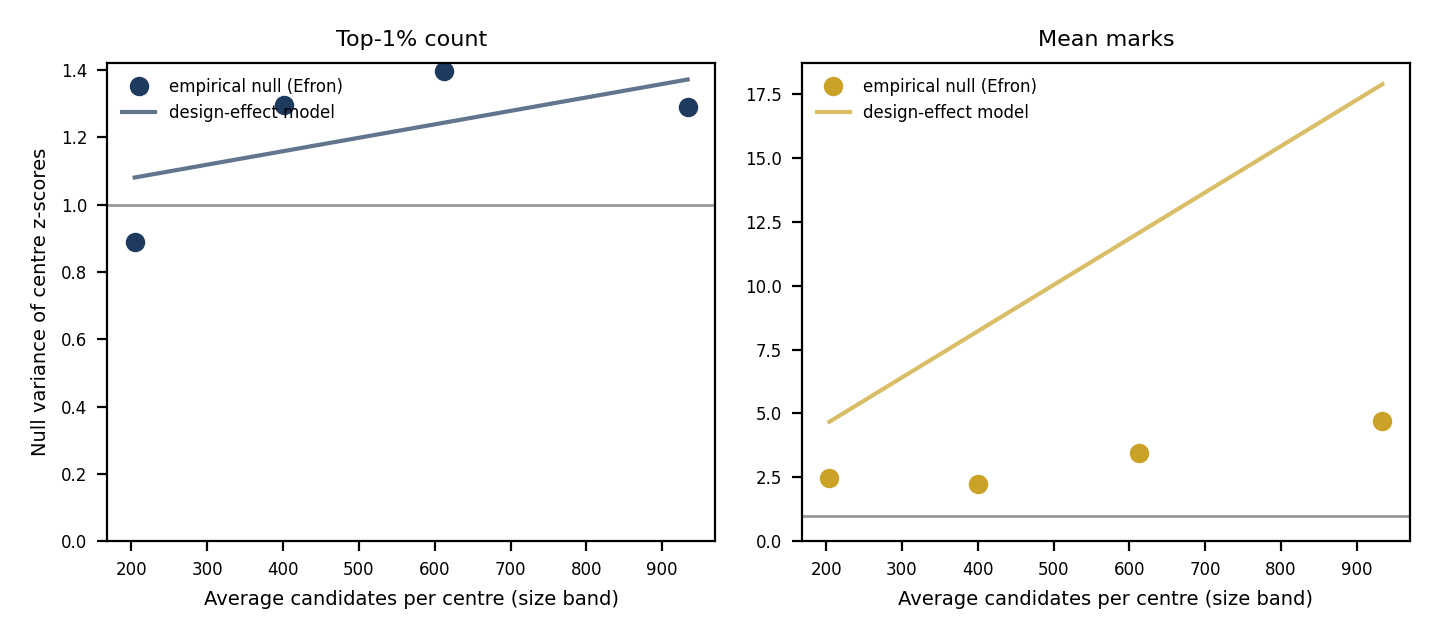
\includegraphics[width=0.78\linewidth]{screen_null_by_size.png}
\caption{Null variance of centre z-scores by centre size. Points: Efron's empirical null. Lines: the design-effect model. For top-1\% counts the model fits; for mean marks the empirical core is narrower than the model, because grouping is concentrated in some states (Section~\ref{sec:states}).}\label{fig:null}
\end{figure}

\subsection{Nine flags, all stronger cohorts}
The screen flags \FlagsLayerTwo{} centres for more top-1\% scorers than random allotment allows after the design effect (Table~\ref{tab:flags}); the exact test without it flags \FlagsLayerOne. Six are in Haryana and three in Gujarat. All \FlagsLowerHalfShiftPositive{} are shifted at their 10th and 25th percentiles too, by a median of \FlagsLowerHalfShiftMedian{} marks (Figure~\ref{fig:profiles}). At Delhi Public School, Rewari, the median candidate scored \ProfRewariOwnMedian{} against \ProfRewariRestMedian{} in the rest of the city. Stronger cohorts allotted together produce this pattern; a boost to some candidates does not.

Under the tail-beyond-bulk test, \TailFlagsOfRegistered{} of the \FlagsLayerTwo{} flags remains. Six have fewer top scorers than their own bulk predicts. Across \StabSeeds{} seeds, \StabRegisteredAllSeeds{} flags hold every time and the weakest holds \StabRegisteredMinRate{} of the time.

\begin{table}[htbp]\centering
\caption{Registered flags: centres with more top-1\% scorers than random allotment within their city allows ($q \le 0.05$ after the design effect). Exp.: expected count under random allotment. Seeds: share of \StabSeeds{} seeds that flag the centre. Shift: mean shift of the 10th and 25th percentiles against the rest of the city, in marks. Bulk: top-1\% count predicted by the centre's own middle half. Tail $z$: observed against that prediction (Addition A1).}\label{tab:flags}
{\scriptsize
\setlength{\tabcolsep}{4pt}
\resizebox{\linewidth}{!}{\begin{tabular}{p{4.6cm}lrrrrrrrrr}
\toprule
Centre & City & $n$ & Top 1\% & Exp. & $z_{adj}$ & $q$ & Seeds & Shift & Bulk & Tail $z$ \\
\midrule
Unit-1 School Of Engineering R.K. University & Rajkot & 1,968 & 93 & 38.2 & 7.31 & $<$0.0001 & 100\% & +38 & 34.7 & 8.33 \\
Rao Pahlad Singh Sr. Sec. School & Mahendragarh & 448 & 34 & 13.4 & 5.02 & 0.0006 & 100\% & +21 & 49.4 & -2.50 \\
Shankersinh Vaghela Bapu Institute Of Technology & Gandhinagar & 1,165 & 23 & 10.0 & 4.24 & 0.017 & 100\% & +18 & 7.8 & 4.43 \\
Delhi Public School, Rewari & Rewari & 264 & 21 & 7.6 & 4.15 & 0.019 & 100\% & +74 & 33.9 & -2.58 \\
Yaduvanshi Shiksha Niketan & Gurugram & 271 & 19 & 6.3 & 4.06 & 0.022 & 100\% & +14 & 31.0 & -2.38 \\
DAV Police Public School & Hissar & 434 & 29 & 12.1 & 4.03 & 0.022 & 100\% & +43 & 38.2 & -1.58 \\
DAV Police Public School & Bhiwani & 328 & 20 & 7.6 & 3.78 & 0.044 & 72\% & +27 & 20.0 & 0.10 \\
Delhi World Public School & Bhiwani & 397 & 22 & 9.2 & 3.77 & 0.044 & 18\% & +62 & 36.7 & -2.79 \\
Shri Vividhlaxi Vidyamandir Palanpur & Banaskantha & 544 & 13 & 3.7 & 3.76 & 0.044 & 56\% & +2 & 11.7 & 0.48 \\
\bottomrule
\end{tabular}}}

\end{table}

\begin{figure}[htbp]\centering
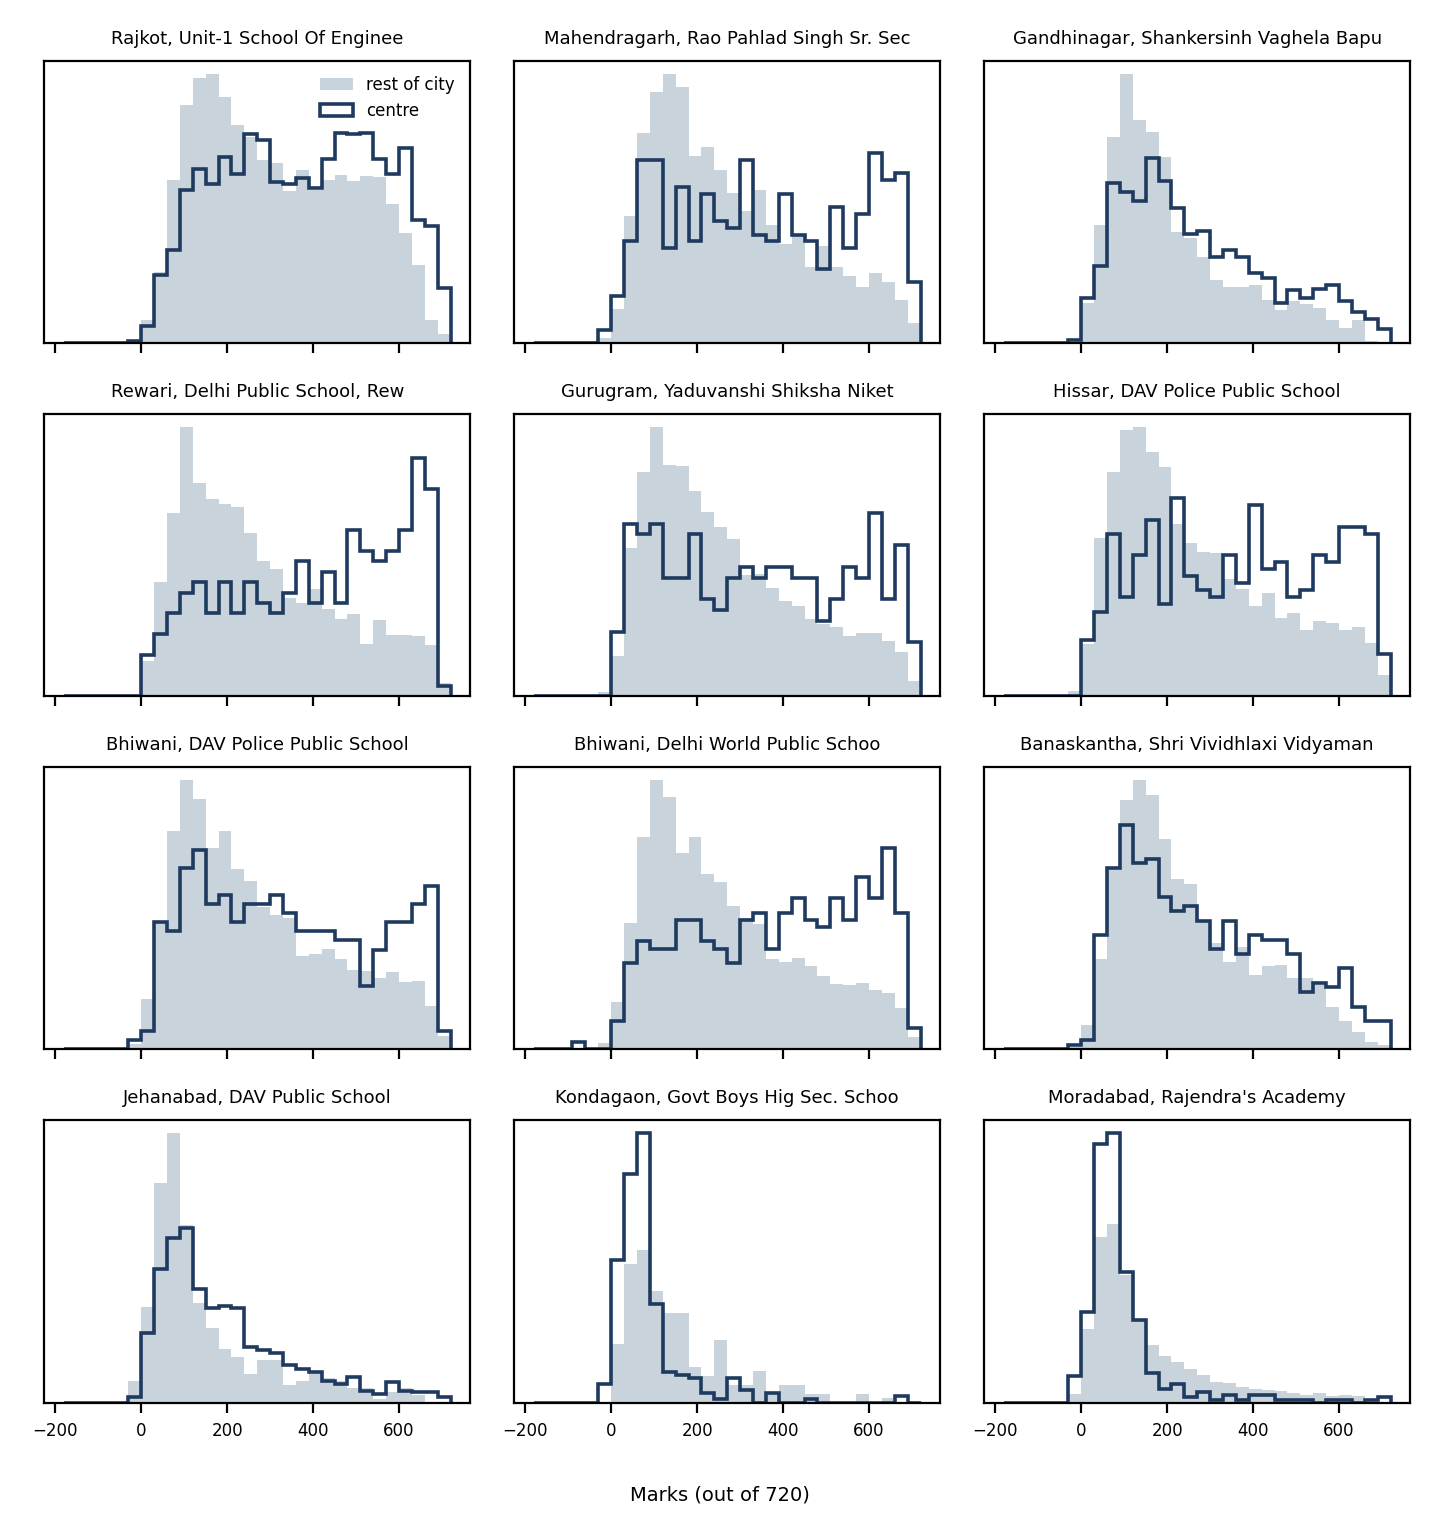
\includegraphics[width=0.95\linewidth]{flag_profiles.png}
\caption{Every flagged centre (line) against the rest of its city (bars). The first nine are the registered flags: whole distributions shifted upwards. The last three are flagged only by the tail-beyond-bulk test.}\label{fig:profiles}
\end{figure}

\paragraph{R.K. University Unit-1, Rajkot.} One centre is anomalous on both counts, under every seed. It has \TailRkK{} top-1\% scorers where random allotment within Rajkot predicts \TailRkEOne{} and its own bulk predicts \TailRkE. It is the largest centre in the data. Its candidates are also stronger overall (median \RkOwnMedian{} against \RkRestMedian{} in the rest of Rajkot), and its very top is not unusually extreme: \RkTopZeroOneShareOfTopOne{} of its top-1\% scorers reach 699 or more, against \NatTopZeroOneShareOfTopOne{} nationally (p \RkPExtreme). The press singled this centre out in July 2024 using the same data. Two readings fit the totals equally well: a strong sub-cohort allotted together (for example from one coaching programme, or one paper medium in a city where many take Gujarati) or a boost to some candidates. Only item-level answer data, which NTA holds, can separate them. This report makes no finding of misconduct.

\paragraph{Deficits.} The screen also finds \DeficitsLayerTwo{} centres with far fewer top scorers than their city: Bhartiya Public School in Sikar (median \ProfSikarbpsOwnMedian{} against \ProfSikarbpsRestMedian) and Trinity International School in Namakkal (\ProfNamakkaltisOwnMedian{} against \ProfNamakkaltisRestMedian). Both cities are coaching hubs, which suggests weaker cohorts grouped away from coaching students.

\subsection{The blind test: incident centres look ordinary}
Every centre on the blind list behaves as predicted (Table~\ref{tab:blind}). None of the \ValListANamed{} named incident centres is flagged for excess or deficit; on average they rank above only \ValListANamedMeanCityPercentile{} of the other centres in their city. Oasis School, where the paper leaked, has \ValTwoSixZeroFourZeroTwoTopOne{} top scorers against \ValTwoSixZeroFourZeroTwoEOne{} expected. The Godhra centre, where the plot was foiled and the suspects' results withheld, has \ValTwoTwoZeroFiveZeroTwoTopOne{} against \ValTwoTwoZeroFiveZeroTwoEOne.

The leak's beneficiaries did not score like toppers. Hazaribagh has \CourtHazaribaghTopOne{} candidates in the national top 1\% and \CourtHazaribaghTopZeroOne{} in the top 0.1\%, so at most \CourtHazaribaghTopOne{} of the roughly 125 beneficiaries reached the top 1\%. On the between-city funnel, Hazaribagh ranks \CourtHazaribaghFunnelRank{} of \FunnelCities{} cities ($z$ = \CourtHazaribaghZFunnel), Patna \CourtPatnaFunnelRank{} ($z$ = \CourtPatnaZFunnel) and Godhra \CourtGodhraFunnelRank{} ($z$ = \CourtGodhraZFunnel).

\begin{table}[htbp]\centering
\caption{The blind list, compiled before marks were analysed. List A: centres in the court and investigation record (Dantewada and Tura are ambiguous: sources do not say which of the city's centres was affected). List B: centres singled out in the press after the release (not blind). In city: rank of the centre's $z$ among its city's centres.}\label{tab:blind}
{\scriptsize
\setlength{\tabcolsep}{4pt}
\resizebox{\linewidth}{!}{\begin{tabular}{lp{4.2cm}lp{2.6cm}rrrrrr}
\toprule
 & Centre & City & Incident & Top 1\% & Exp. & $z_{adj}$ & $q$ & Tail $z$ & In city \\
\midrule
A & Oasis School & Hazaribagh & Leak origin & 5 & 4.6 & 0.03 & 1.000 & 0.97 & 2 of 5 \\
A & Jay Jalaram School & Godhra & Foiled insider plan & 0 & 1.0 & -1.76 & 1.000 & -0.70 & 2 of 2 \\
A & Balika Ucch Madhyamik Adarsh Vidhya Mandir & Sawai Madhopur & Wrong-medium papers & 7 & 6.7 & 0.33 & 1.000 & -0.49 & 2 of 6 \\
A & Hardayal Public School & Jhajjar & Grace marks, re-test & 2 & 4.3 & -1.06 & 1.000 & -0.71 & 2 of 3 \\
A & Govt.Boys Adarsh Hr.Sec.School Balod & Balod & Grace marks, re-test & 0 & 0.0 & -1.15 & 1.000 & -2.98 & 2 of 2 \\
A & Govt. Danteshwari P.G. College, Dantewada (C.G.) & Dantewada & Grace marks (one of two) & 0 & 0.0 & -1.97 & 1.000 & -3.08 & 2 of 2 \\
A & Swami Atmanand Govt. Utkrisht Hindi Medium Higher Secondary School Dantewada & Dantewada & Grace marks (one of two) & 0 & 0.0 & 1.13 & 1.000 & -0.33 & 1 of 2 \\
A & Government Boys Higher Secondary School & Tura & Grace marks (one of three) & 0 & 0.0 & -0.16 & 1.000 & -0.63 & 2 of 3 \\
A & Montfort School & Tura & Grace marks (one of three) & 0 & 0.0 & 0.48 & 1.000 & -3.53 & 1 of 3 \\
A & Capt William's Sch Matchakolgre & Tura & Grace marks (one of three) & 0 & 0.0 & -0.18 & 1.000 & 0.14 & 3 of 3 \\
B & Unit-1 School Of Engineering R.K. University & Rajkot & Singled out in press & 93 & 38.2 & 7.31 & $<$0.0001 & 8.33 & 1 of 7 \\
B & (Unit-2) School Of Engineering, R.K. University & Rajkot & Singled out in press & 10 & 18.9 & -1.94 & 1.000 & -2.25 & 5 of 7 \\
\bottomrule
\end{tabular}}}

\end{table}

\subsection{What the screen can and cannot catch}
A boost to a few per cent of one centre's candidates is caught reliably (Table~\ref{tab:injectc}). At 80\% detection the screen needs about \InjectMinMEightZeroLTwoTwoFiveZero{} boosted candidates at centres under 250, \InjectMinMEightZeroLTwoTwoFiveZeroFourNineNine{} at 250-499, \InjectMinMEightZeroLTwoFiveZeroZeroSevenFourNine{} at 500-749 and \InjectMinMEightZeroLTwoSevenFiveZero{} at 750 or more. The tail-beyond-bulk test is weaker for large boosts, because a large boost also lifts the bulk; that is the price of its specificity.

A leak spread across a city is a different matter (Table~\ref{tab:injectl}). Within-city tests catch it at the false-positive rate, because they compare each centre with a city that has been lifted too. Only the between-city funnel sees city leaks, and only large ones relative to the city. Had Hazaribagh's roughly 125 beneficiaries scored like the national top 1\%, the funnel would have caught it in \InjectHazaribaghOneTwoFiveFunnel{} of simulations; had they scored like the top 10\%, in \InjectHazaribaghTopOneZeroOneTwoFiveFunnel. A Patna-scale leak of 30 among \GeoPatnaN{} candidates is invisible to every test here.

\begin{table}[htbp]\centering
\caption{Centre fraud: share of 400 injections detected, by number of boosted candidates and centre size. Each cell: registered screen / tail beyond the bulk.}\label{tab:injectc}
{\small
\begin{tabular}{lrrrr}
\toprule
Boosted candidates & under 250 & 250-499 & 500-749 & 750 or more \\
\midrule
5 & 16\% / 20\% & 4\% / 10\% & 2\% / 3\% & 2\% / 6\% \\
10 & 84\% / 50\% & 49\% / 34\% & 24\% / 15\% & 14\% / 12\% \\
20 & 100\% / 78\% & 96\% / 67\% & 87\% / 54\% & 71\% / 47\% \\
40 & 100\% / 66\% & 100\% / 90\% & 100\% / 89\% & 98\% / 89\% \\
80 & 100\% / 48\% & 100\% / 73\% & 100\% / 96\% & 100\% / 99\% \\
\bottomrule
\end{tabular}}

\end{table}

\begin{table}[htbp]\centering
\caption{City leaks: share of 400 injections detected. ``A random city'' is drawn from cities with at least five times as many candidates as beneficiaries. Beneficiaries' marks are drawn from the national top 1\% unless the scenario says top 10\%. The funnel counts a detection only when the city was not already above its upper limit.}\label{tab:injectl}
{\small
\setlength{\tabcolsep}{4pt}
\resizebox{\linewidth}{!}{\begin{tabular}{lrrrr}
\toprule
Scenario & Beneficiaries & Within-city screen & Tail beyond bulk & City funnel \\
\midrule
A random city & 25 & 2\% & 8\% & 20\% \\
A random city & 50 & 1\% & 15\% & 50\% \\
A random city & 100 & 0\% & 22\% & 75\% \\
A random city & 200 & 0\% & 24\% & 91\% \\
Hazaribagh, top 1\% & 125 & 0\% & 0\% & 100\% \\
Hazaribagh, top 10\% & 125 & 0\% & 0\% & 0\% \\
Patna, top 1\% & 30 & 0\% & 0\% & 0\% \\
Patna, top 10\% & 30 & 0\% & 0\% & 0\% \\
\bottomrule
\end{tabular}}}

\end{table}

\subsection{Where allotment departs from a lottery, and why it matters}\label{sec:states}
The grouping of average marks is not spread evenly across India (Figure~\ref{fig:states}). In \MediumLotteryLikeStates{} of \MediumStates{} states with ten or more testable centres, centre means behave almost exactly like random draws from their city (standard deviation of centre z-scores under 1.5). In \MediumSortedStates{} they are strongly grouped (above 3); in Madhya Pradesh the ICC of marks is \StateMadhyapradeshIcc{} and the standard deviation \StateMadhyapradeshSdz.

Paper medium is the leading explanation. NTA prints a different booklet for each medium and offers regional media only in their own states (NTA 2023). Across the \MediumRegionalStates{} states that offer a regional-language paper, the share of registrants choosing one predicts the ICC (Spearman \MediumSpearman, p = \MediumSpearmanP). Gujarat (\StateGujaratRegshare{} regional), West Bengal (\StateWestbengalRegshare), Tamil Nadu (\StateTamilnaduRegshare) and Assam (\StateAssamRegshare) are the four most grouped of the twelve; Kerala, Karnataka, Maharashtra, Odisha, Andhra Pradesh, Telangana and Punjab, all under 2\%, are close to a lottery (ICC under 0.003). NTA gives no state split for Hindi; most Hindi-belt states are strongly grouped. This analysis was added after the first results (Addition A2) and rests on state-level shares, so it is suggestive, not proof.

It matters for two reasons. Grouping makes centre-level screening noisier where it is strongest. And it makes allotment predictable: a candidate who knows the rule can choose a city and medium served by few centres and know roughly where they will sit. Godhra shows how little choice is needed: its only two centres belonged to the school group behind the foiled 2024 plot.

\begin{figure}[htbp]\centering
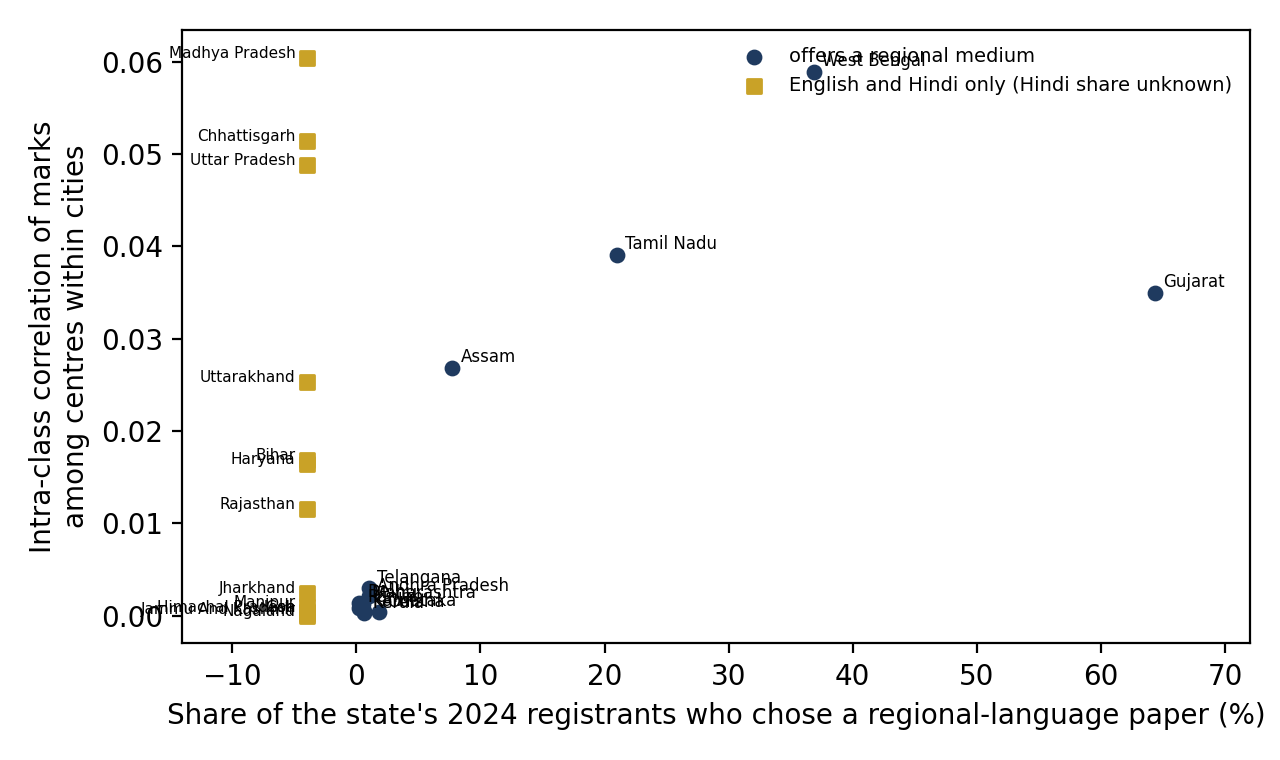
\includegraphics[width=0.98\linewidth]{state_allotment.png}
\caption{How far allotment departs from a lottery, by state (left), against the share of 2024 registrants who chose a regional-language paper (right).}\label{fig:states}
\end{figure}

\subsection{Serial numbers are shuffled}
If NTA's serial numbers followed seating order, room-sized clusters of top scorers could be screened for. They do not. The lag-1 autocorrelation of marks along serial order is indistinguishable from a random shuffle in \SerialCentres{} centres (pooled $z$ = \SerialPooledZ; standard deviation of centre z-scores \SerialSdZ), and at every lag from 1 to 30. Genuine permutation tests on 100 centres confirm the calibration. The registered pathway for this case applies: no room-level analysis is possible with the public data.

\section{Geography}\label{sec:geo}
Top scores are concentrated. Ten cities hold \GeoTopOneZeroShareTopOne{} of the national top 1\% with \GeoTopOneZeroShareCandidates{} of candidates. Sikar alone has \GeoSikarTopOne{} top-1\% scorers from \GeoSikarN{} candidates (\GeoSikarRate), more than Delhi's \GeoDelhiTopOne{} from \GeoDelhiN.

City rates vary far more than chance allows: without an allowance for overdispersion, \GeoPlainOutsideNineNineEight{} of \GeoCities{} cities would fall outside 99.8\% funnel limits. With it (Spiegelhalter 2005), \GeoHubs{} hub cities remain above the upper limit (Figure~\ref{fig:funnel}, Table~\ref{tab:hubs}). They hold \GeoHubCandidatesShare{} of candidates and \GeoHubTopOneShare{} of top scorers; eight are in Rajasthan and five in Haryana. In half of them the excess is spread evenly across centres, as a coaching ecosystem would produce (Kottayam, Malappuram, Jaipur). In the other half it is concentrated in some centres (Sikar, Kota, Namakkal and most Haryana hubs), which matches the grouping found above.

\begin{figure}[htbp]\centering
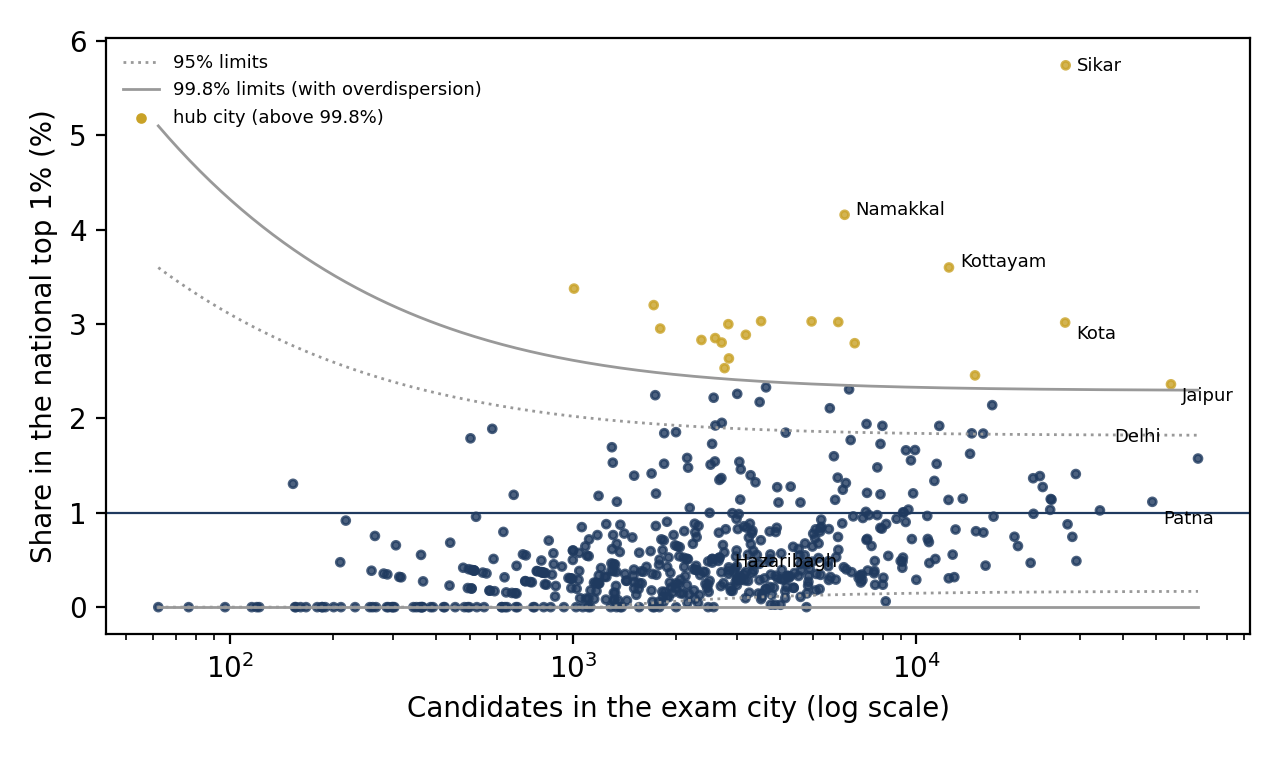
\includegraphics[width=0.85\linewidth]{geo_funnel.png}
\caption{Funnel plot of city top-1\% rates. Limits are widened for between-city overdispersion.}\label{fig:funnel}
\end{figure}

\begin{table}[htbp]\centering
\caption{Hub cities: above the 99.8\% funnel limit after the overdispersion allowance. Across centres: whether the city's centres differ more than random allotment allows (heterogeneity test, $p < 0.05$).}\label{tab:hubs}
{\scriptsize
\setlength{\tabcolsep}{4pt}
\resizebox{\linewidth}{!}{\begin{tabular}{llrrrrrl}
\toprule
City & State & Candidates & Top 1\% & Rate & Funnel $z$ & Centres & Across centres \\
\midrule
Sikar & Rajasthan & 27,216 & 1,563 & 5.7\% & 11.18 & 49 & concentrated \\
Namakkal & Tamil Nadu & 6,180 & 257 & 4.2\% & 7.21 & 11 & concentrated \\
Kottayam & Kerala & 12,443 & 448 & 3.6\% & 6.06 & 31 & even \\
Kota & Rajasthan & 27,118 & 818 & 3.0\% & 4.76 & 56 & concentrated \\
Bikaner & Rajasthan & 5,923 & 179 & 3.0\% & 4.61 & 13 & even \\
Jhunjhunu & Rajasthan & 4,953 & 150 & 3.0\% & 4.58 & 11 & concentrated \\
Sriganganagar & Rajasthan & 1,718 & 55 & 3.2\% & 4.56 & 4 & even \\
Tanuku & Andhra Pradesh & 1,007 & 34 & 3.4\% & 4.54 & 3 & even \\
Chandigarh/Mohali & Chandigarh(Ut) & 3,530 & 107 & 3.0\% & 4.50 & 4 & even \\
Mahendragarh & Haryana & 2,834 & 85 & 3.0\% & 4.36 & 5 & concentrated \\
Rewari & Haryana & 3,187 & 92 & 2.9\% & 4.15 & 9 & concentrated \\
Hissar & Haryana & 6,613 & 185 & 2.8\% & 4.12 & 14 & concentrated \\
Kurukshetra & Haryana & 1,795 & 53 & 3.0\% & 4.07 & 4 & even \\
Jajpur & Odisha & 2,595 & 74 & 2.9\% & 4.01 & 6 & even \\
Karnal & Haryana & 2,366 & 67 & 2.8\% & 3.93 & 6 & concentrated \\
Bhatinda & Punjab & 2,710 & 76 & 2.8\% & 3.92 & 6 & even \\
Baran & Rajasthan & 2,845 & 75 & 2.6\% & 3.57 & 7 & concentrated \\
Malappuram & Kerala & 14,818 & 364 & 2.5\% & 3.41 & 30 & even \\
Churu & Rajasthan & 2,763 & 70 & 2.5\% & 3.34 & 8 & concentrated \\
Jaipur & Rajasthan & 55,124 & 1,302 & 2.4\% & 3.23 & 86 & even \\
\bottomrule
\end{tabular}}}

\end{table}

Development explains who qualifies, not who tops (Figure~\ref{fig:dev}, Table~\ref{tab:dev}). Across \GeoUnits{} district units, the development index correlates with mean marks at \GeoDevMeanMarksRho{} (95\% interval \GeoDevMeanMarksLo{} to \GeoDevMeanMarksHi) and with the share at or above the median at \GeoDevGeMedShareRho, but with the top-1\% share at only \GeoDevTopOneRateRho{} (\GeoDevTopOneRateLo{} to \GeoDevTopOneRateHi). The registered prediction (positive for all three) holds. The weakness at the top survives every sensitivity run. Of the districts, \GeoPdPositive{} sit more than two standard deviations above their development-predicted top-1\% rate; Bikaner, Baran and Jajpur are hubs despite below-average development. These are correlations between places, not people (Robinson 1950), and an exam city is not a candidate's home district.

\begin{figure}[htbp]\centering
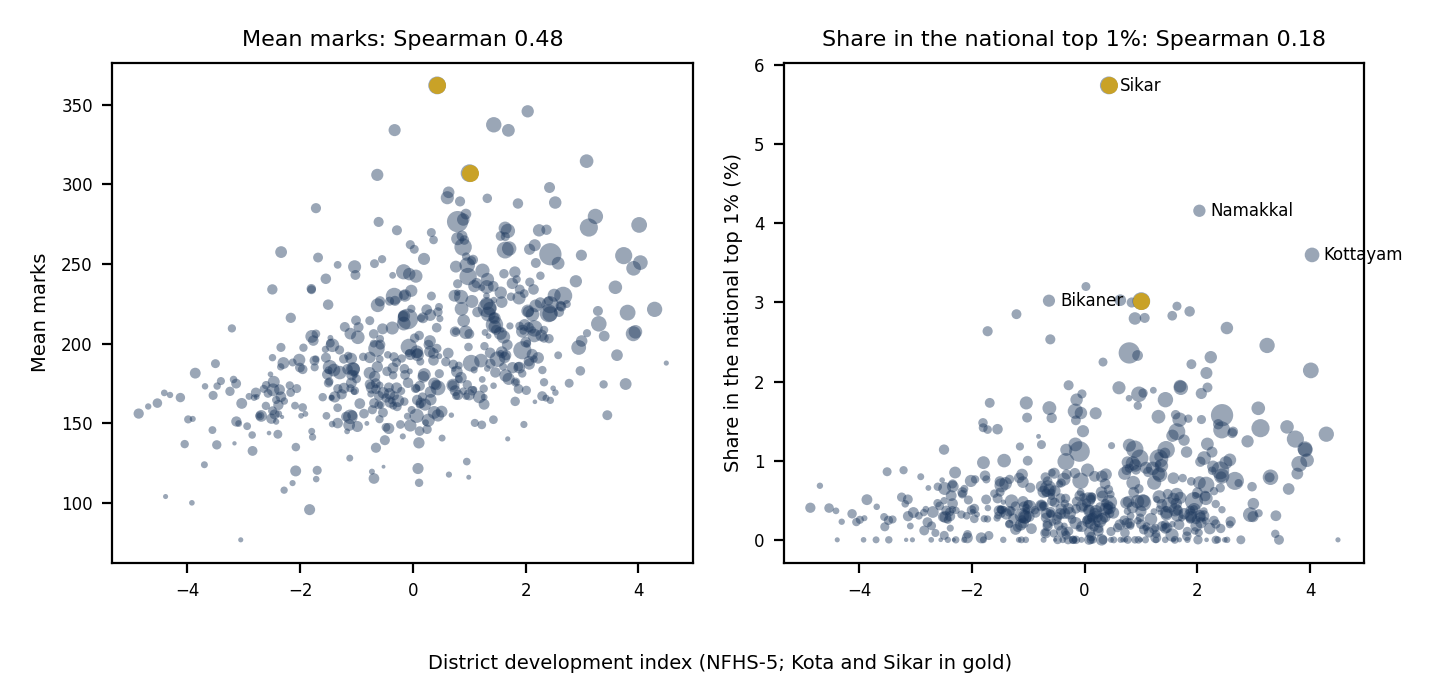
\includegraphics[width=0.95\linewidth]{geo_development.png}
\caption{District development against mean marks (left) and the share in the national top 1\% (right). Point size: candidates.}\label{fig:dev}
\end{figure}

\begin{table}[htbp]\centering
\caption{Spearman correlation of the development index with each outcome, with 95\% bootstrap intervals (2,000 resamples).}\label{tab:dev}
{\scriptsize
\begin{tabular}{lllll}
\toprule
Outcome & All units & Certain mappings & Without Kota, Sikar & 1,000+ candidates \\
\midrule
Mean marks & 0.48 [0.41, 0.54] & 0.47 [0.41, 0.53] & 0.48 [0.41, 0.54] & 0.46 [0.38, 0.53] \\
Share at or above the median & 0.51 [0.44, 0.57] & 0.50 [0.44, 0.56] & 0.51 [0.44, 0.57] & 0.49 [0.42, 0.55] \\
Share in the top 1\% & 0.18 [0.09, 0.26] & 0.17 [0.08, 0.25] & 0.18 [0.09, 0.26] & 0.18 [0.09, 0.27] \\
\bottomrule
\end{tabular}}

\end{table}

\section{Rank fragility}\label{sec:fragility}
A NEET rank is finer than the measurement behind it. At 577 marks, the score at rank 108,000 that the court used as its seat line, one question (5 marks, wrong instead of right) moves a candidate \FrFiveSevenSevenRanksFive{} places, and \FrWithinFiveOfFiveSevenSeven{} candidates sit within five marks of the line (Table~\ref{tab:frag}, Figure~\ref{fig:frag}). At exactly 600 marks, \FrSixZeroZeroTie{} candidates share one total, ordered only by the tie-break rules (Biology, then Chemistry, then Physics, then fewer wrong answers; NTA dropped age and lottery for 2024).

The 26 July revision of one physics question took 5 marks from about four lakh candidates (Business Today 2024), \FrRevisedShare{} of those who appeared. If they were spread evenly, a candidate at 577 who lost the marks fell about \FrFiveSevenSevenRevisionLossIfHit{} places, and one who kept them rose about \FrFiveSevenSevenRevisionGainIfSpared.

Lord's binomial error model (Lord 1965) gives an illustrative sense of measurement noise. If a candidate at 577 attempted all 180 questions, one standard error on a parallel paper is about \FrFiveSevenSevenSem{} marks, ranks \FrFiveSevenSevenBandBest{} to \FrFiveSevenSevenBandWorst. This is an upper estimate: questions differ in difficulty, and candidates who leave questions blank have narrower bands.

The distribution also shows how many candidates guess. A candidate who attempts all 180 questions scores $5c - 180$, a multiple of 5, so guessing leaves a comb in the histogram. About \CombLow{} of the lowest scorers attempted every question, against \CombMid{} in the middle of the distribution (Addition A3).

\begin{figure}[htbp]\centering
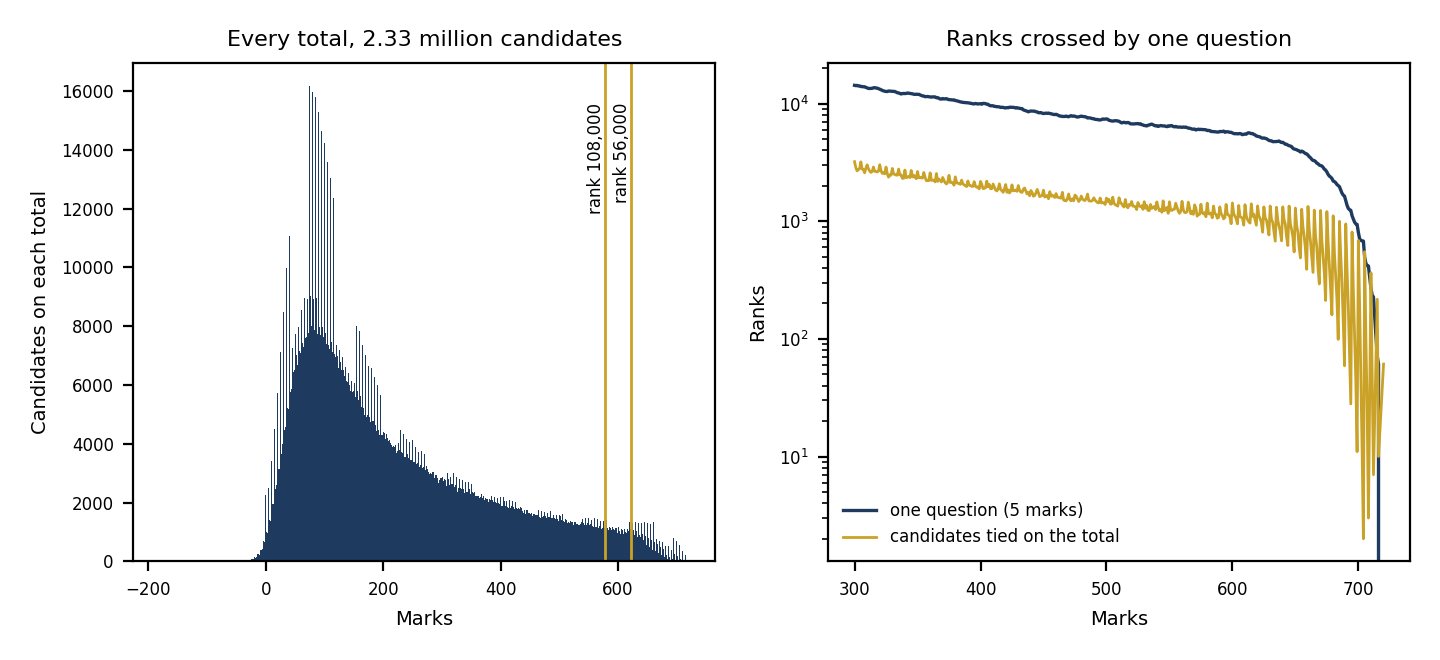
\includegraphics[width=0.98\linewidth]{fragility.png}
\caption{Left: candidates on every total. Right: ranks crossed by one question, and candidates tied on each total.}\label{fig:frag}
\end{figure}

\begin{table}[htbp]\centering
\caption{Ranks at key scores. 1, 4 and 5 marks: ranks crossed by a blank instead of a wrong answer, a right answer instead of a blank, and a right answer instead of a wrong one. SEM: Lord's binomial standard error if all 180 questions were attempted (an upper estimate).}\label{tab:frag}
{\small
\begin{tabular}{rrrrrrrr}
\toprule
Marks & Best rank & Tied on it & 1 mark & 4 marks & 5 marks & SEM & Ranks within one SEM \\
\midrule
450 & 286,419 & 1,834 & 1,604 & 6,434 & 8,217 & 31 & 237,073 to 341,892 \\
550 & 140,654 & 1,461 & 1,235 & 4,993 & 6,414 & 26 & 108,156 to 174,917 \\
577 & 107,004 & 1,152 & 1,184 & 4,854 & 6,006 & 25 & 77,859 to 138,184 \\
600 & 80,123 & 1,428 & 1,163 & 4,261 & 5,621 & 23 & 54,777 to 107,004 \\
622 & 55,748 & 1,057 & 971 & 4,171 & 5,195 & 21 & 35,257 to 78,960 \\
650 & 28,911 & 1,294 & 919 & 2,811 & 4,074 & 18 & 15,515 to 45,537 \\
680 & 8,398 & 1,111 & 539 & 1,197 & 2,194 & 14 & 3,558 to 16,514 \\
700 & 1,636 & 686 & 195 & 253 & 803 & 10 & 341 to 4,244 \\
\bottomrule
\end{tabular}}

\end{table}

\section{Deployment}\label{sec:deploy}
\paragraph{The integrity monitor.} \texttt{fairexams.monitor} runs the whole screen on any exam's centre-wise results: a CSV with one row per candidate and three columns (centre, city, marks). It reports every centre's exact and design-effect tests, false discovery rates, the tail-beyond-bulk test and flag stability across seeds, with a plain-language summary that states what a flag does and does not mean. On a synthetic exam of \DemoCandidates{} candidates in \DemoCities{} cities, half of them grouping candidates into stronger and weaker centres, with 30 boosted candidates at one centre, the monitor flags the planted centre on both lists under every seed ($z$ = \DemoPlantedZ{} and \DemoPlantedZtail). It flags one grouped strong cohort on the first list only. The exact test without the design effect would have raised \DemoFlagsExact{} alarms. On NEET 2024 it reproduces the registered flags.

\paragraph{The explorer.} \texttt{docs/index.html} is a single offline page with every centre, city and state: any centre against its city, the flags with their stability, hub cities and allotment by state. It holds aggregates only.

\paragraph{Five recommendations.}
\begin{enumerate}[leftmargin=1.5em]
\item \textbf{Publish centre-wise results every year.} The 2024 release let anyone check the figures the court relied on; this audit reproduces them exactly. Without such a release, none of this is possible for 2025 or 2026.
\item \textbf{Randomise allotment within medium, record the seed, publish the rule.} Allot each candidate at random among all centres in the city that can serve their medium, avoid serving a medium from a single centre in a city, and avoid cities whose centres all belong to one institution. This removes the predictability a plotter needs and makes every centre a valid random sample.
\item \textbf{Run answer-similarity checks on item-level data.} Totals cannot see a leak sold across a city, and cannot tell a strong cohort from a boosted one. Shared wrong answers can. Methods exist (Wollack 1997; van der Linden and Sotaridona 2006); only NTA holds the response data.
\item \textbf{Publish a room identifier.} A shuffled serial number hides seating. A coarse room code would allow room-level screening without identifying anyone.
\item \textbf{Pre-register the monitoring rule.} Fix the statistics, thresholds and false discovery rate before results are out, so flags trigger review automatically and cannot be chosen after the fact.
\end{enumerate}

\section{Limitations}\label{sec:limits}
\begin{itemize}[leftmargin=1.2em]
\item Totals only. Without item responses, a strong cohort and a boosted one look alike, and leaks spread across a city are invisible within it.
\item The design-effect allowance assumes one national $\rho$ for top-1\% status. Grouping is uneven across states, so screening is noisier where grouping is strongest.
\item The medium explanation rests on state-level shares, with no state split for Hindi. It is suggestive.
\item District development refers to the exam city's district, not candidates' homes, and NFHS-5 predates the exam by three to five years.
\item The rank analysis uses the pre-revision file; Lord's band is an illustration under stated assumptions.
\item Every number is regenerated by the pipeline from public data, but the work has not been peer reviewed.
\end{itemize}

\section{Reproducibility}
Every number in this report is written by the pipeline into \nolinkurl{results/numbers.json} and \nolinkurl{report/numbers.tex}; none is typed by hand. \texttt{make all} downloads the data, verifies it against NTA's PDFs, rebuilds every panel, reruns every analysis with fixed seeds and recompiles this report. Raw data is never redistributed. Code is MIT-licensed.

\section*{References}
\begin{small}
\begin{itemize}[leftmargin=1em,label={}]
\item Benjamini, Y. and Hochberg, Y. (1995). Controlling the false discovery rate: a practical and powerful approach to multiple testing. \textit{Journal of the Royal Statistical Society B} 57(1): 289-300.
\item Business Today (2024). SC on NEET UG 2024: 4 lakh students to lose 5 marks each. 24 July 2024.
\item Christiansen, J. L. et al.\ (2013). Measuring transit signal recovery in the Kepler pipeline. I. Individual events. \textit{Astrophysical Journal Supplement} 207: 35.
\item Cizek, G. J. and Wollack, J. A., eds.\ (2017). \textit{Handbook of Quantitative Methods for Detecting Cheating on Tests}. Routledge.
\item DerSimonian, R. and Laird, N. (1986). Meta-analysis in clinical trials. \textit{Controlled Clinical Trials} 7(3): 177-188.
\item Efron, B. (2004). Large-scale simultaneous hypothesis testing: the choice of a null hypothesis. \textit{Journal of the American Statistical Association} 99(465): 96-104.
\item Efron, B. (2010). \textit{Large-Scale Inference}. Cambridge University Press.
\item Fisher, R. A. (1935). \textit{The Design of Experiments}. Oliver and Boyd.
\item Geyer, C. J. and Meeden, G. D. (2005). Fuzzy and randomized confidence intervals and p-values. \textit{Statistical Science} 20(4): 358-366.
\item IIPS and ICF (2021). \textit{National Family Health Survey (NFHS-5), 2019-21}. International Institute for Population Sciences, Mumbai.
\item Jacob, B. A. and Levitt, S. D. (2003). Rotten apples: an investigation of the prevalence and predictors of teacher cheating. \textit{Quarterly Journal of Economics} 118(3): 843-877.
\item Kish, L. (1965). \textit{Survey Sampling}. Wiley.
\item Kulldorff, M. (1997). A spatial scan statistic. \textit{Communications in Statistics: Theory and Methods} 26(6): 1481-1496.
\item Lancaster, H. O. (1961). Significance tests in discrete distributions. \textit{Journal of the American Statistical Association} 56(294): 223-234.
\item Lord, F. M. (1965). A strong true-score theory, with applications. \textit{Psychometrika} 30(3): 239-270.
\item Marsh, D. R., Schroeder, D. G., Dearden, K. A., Sternin, J. and Sternin, M. (2004). The power of positive deviance. \textit{BMJ} 329: 1177-1179.
\item National Testing Agency (2023). Public notice: clarification regarding the medium of the question paper for NEET (UG)-2023. 19 April 2023.
\item National Testing Agency (2024). Press release: NTA declares the re-revised result of NEET (UG)-2024. 26 July 2024.
\item Robinson, W. S. (1950). Ecological correlations and the behavior of individuals. \textit{American Sociological Review} 15(3): 351-357.
\item Rosenbaum, P. R. (2002). \textit{Observational Studies}, 2nd ed. Springer.
\item Spiegelhalter, D. J. (2005). Funnel plots for comparing institutional performance. \textit{Statistics in Medicine} 24(8): 1185-1202.
\item Spiegelhalter, D., Sherlaw-Johnson, C., Bardsley, M., Blunt, I., Wood, C. and Grigg, O. (2012). Statistical methods for healthcare regulation: rating, screening and surveillance. \textit{Journal of the Royal Statistical Society A} 175(1): 1-47.
\item Storey, J. D. (2002). A direct approach to false discovery rates. \textit{Journal of the Royal Statistical Society B} 64(3): 479-498.
\item Supreme Court of India (1970). \textit{Bihar School Examination Board v. Subhas Chandra Sinha}, (1970) 1 SCC 648.
\item Supreme Court of India (2024). \textit{Vanshika Yadav v. Union of India}, 2024 INSC 568, judgment of 2 August 2024.
\item van der Linden, W. J. and Sotaridona, L. (2006). Detecting answer copying when the regular response process follows a known response model. \textit{Journal of Educational and Behavioral Statistics} 31(3): 283-304.
\item Wollack, J. A. (1997). A nominal response model approach for detecting answer copying. \textit{Applied Psychological Measurement} 21(4): 307-320.
\end{itemize}
\end{small}

\appendix
\section{Allotment by state}
\begin{table}[H]\centering
\caption{States with ten or more testable centres. ICC of marks among centres within cities; standard deviation of centre-mean z-scores (1 under random allotment); share of centres beyond $\pm3$; share of registrants choosing a regional-language paper.}
{\scriptsize
\begin{tabular}{lrrrrr}
\toprule
State & Centres & ICC of marks & SD of centre $z$ & $|z|>3$ & Regional-medium share \\
\midrule
Madhya Pradesh & 280 & 0.0604 & 5.66 & 84\% & Hindi/English \\
West Bengal & 223 & 0.0589 & 5.61 & 77\% & 36.8\% \\
Chhattisgarh & 92 & 0.0514 & 5.38 & 84\% & Hindi/English \\
Uttar Pradesh & 598 & 0.0488 & 5.55 & 75\% & Hindi/English \\
Tamil Nadu & 270 & 0.0391 & 4.74 & 54\% & 21.0\% \\
Gujarat & 178 & 0.0350 & 4.29 & 43\% & 64.3\% \\
Assam & 95 & 0.0269 & 3.55 & 26\% & 7.7\% \\
Uttarakhand & 40 & 0.0254 & 3.98 & 38\% & Hindi/English \\
Bihar & 221 & 0.0168 & 3.59 & 33\% & Hindi/English \\
Haryana & 128 & 0.0164 & 2.72 & 12\% & Hindi/English \\
Rajasthan & 391 & 0.0116 & 2.57 & 15\% & Hindi/English \\
Telangana & 162 & 0.0029 & 1.53 & 4\% & 1.0\% \\
Jharkhand & 65 & 0.0025 & 1.69 & 8\% & Hindi/English \\
Andhra Pradesh & 119 & 0.0021 & 1.39 & 4\% & 1.0\% \\
Delhi & 116 & 0.0014 & 1.34 & 3\% & 0.2\% \\
Maharashtra & 599 & 0.0013 & 1.27 & 2\% & 0.6\% \\
Manipur & 23 & 0.0009 & 1.17 & 0\% & Hindi/English \\
Punjab & 44 & 0.0009 & 1.16 & 0\% & 0.2\% \\
Karnataka & 324 & 0.0005 & 1.10 & 1\% & 0.7\% \\
Himachal Pradesh & 50 & 0.0004 & 1.08 & 0\% & Hindi/English \\
Goa & 16 & 0.0004 & 1.11 & 0\% & Hindi/English \\
Odisha & 148 & 0.0004 & 1.11 & 1\% & 1.8\% \\
Kerala & 302 & 0.0002 & 1.04 & 1\% & 0.6\% \\
Jammu And Kashmir & 107 & 0.0001 & 1.02 & 0\% & Hindi/English \\
Nagaland & 10 & 0.0000 & 1.04 & 0\% & Hindi/English \\
\bottomrule
\end{tabular}}

\end{table}

\section{Additions after the pre-registration}
\begin{itemize}[leftmargin=1.2em]
\item \textbf{A1, tail beyond the bulk.} Designed after seeing that every registered flag is a whole-distribution shift.
\item \textbf{A2, allotment by state and medium.} Designed after seeing the gap between the ICC of marks and of top-1\% status, the coaching-hub deficits, and a Dantewada centre named as a Hindi-medium school scoring below its neighbour.
\item \textbf{A3, the comb.} Seen in the national histogram; descriptive.
\item \textbf{A4, seed stability.} Added when building the monitor showed a borderline flag changing with the random stream.
\end{itemize}
Dates and reasons are in \texttt{DEVIATIONS.md}. No registered analysis was changed or dropped.
\end{document}
